\documentclass{article}
\usepackage{graphicx}
\usepackage{amsmath}
\usepackage{amssymb}
\usepackage{amsthm}
\usepackage{listings}
\usepackage[margin=1in]{geometry}
\usepackage{xcolor}
\usepackage{tikz}
\usetikzlibrary{shapes, arrows, positioning, calc, patterns, decorations.pathreplacing, arrows.meta, matrix, fit}
\usepackage{tcolorbox}
\usepackage{pgfplots}
\pgfplotsset{compat=1.18}
\usepackage{caption}

% Define colors
\definecolor{codegreen}{rgb}{0,0.6,0}
\definecolor{codegray}{rgb}{0.5,0.5,0.5}
\definecolor{codepurple}{rgb}{0.58,0,0.82}
\definecolor{backcolour}{rgb}{0.95,0.95,0.92}
\definecolor{locality}{RGB}{46, 134, 193}
\definecolor{equivariance}{RGB}{52, 152, 219}
\definecolor{invariance}{RGB}{231, 76, 60}
\definecolor{pooling}{RGB}{241, 196, 15}

% Python style
\lstdefinestyle{pythonstyle}{
    backgroundcolor=\color{backcolour},   
    commentstyle=\color{codegreen},
    keywordstyle=\color{magenta},
    numberstyle=\tiny\color{codegray},
    stringstyle=\color{codepurple},
    basicstyle=\ttfamily\footnotesize,
    breakatwhitespace=false,         
    breaklines=true,                 
    captionpos=b,                    
    keepspaces=true,                 
    numbers=left,                    
    numbersep=5pt,                  
    showspaces=false,                
    showstringspaces=false,
    showtabs=false,                  
    tabsize=2
}
\lstset{style=pythonstyle}

% Theorem environments
\newtheorem{theorem}{Theorem}
\newtheorem{principle}{Principle}

\title{From MLPs to CNNs: Why Spatial Structure Matters\\
Understanding Convolution Through Moving Averages and Filters}
\author{Deep Learning Class}
\date{\today}

\begin{document}
\maketitle

\section{The Challenge of Image Recognition}

In the 1980s, machine learning began to revolutionize industries by automating tasks like fraud detection and product recommendations. These models, trained on historical data, often outperformed human experts. However, one task remained stubbornly difficult for traditional machine learning: \textbf{image recognition}. Despite numerous attempts, even complex Multilayer Perceptrons (MLPs) failed to match human-level performance. To understand why, we must first look at how machine learning models work and the unique challenge posed by images.

\subsection{Machine Learning as Curve Fitting}
At its core, machine learning is a form of \textbf{curve fitting}. For a task like distinguishing cats from dogs, we can represent each labeled image as a point on a graph. The input (x-coordinate) represents the image, and the output (y-coordinate) represents its label (e.g., +1 for cat, -1 for dog). The model fits a function to these points to predict the label of a new image. The accuracy of this prediction relies on having a dense collection of labeled points spread throughout the input space.

\subsection{The Curse of Dimensionality}
This approach works well for low-dimensional data. However, images are inherently \textbf{high-dimensional}. A single pixel requires three values for its Red, Green, and Blue (RGB) intensities. A small 32×32 pixel image, therefore, requires $32 \times 32 \times 3 = 3072$ numbers to describe it. For a one-megapixel image, this number grows to three million.

This high dimensionality leads to the ``curse of dimensionality''. As the number of dimensions ($n$) increases, the volume of the input space grows exponentially. To maintain the same density of data points needed for accurate curve fitting, we would need an exponentially larger dataset. For example, if 9 data points are needed to cover a 1D space, we would need $9^2$ for 2D, and $9^n$ points for an n-dimensional space.

For a 32×32 image (3072 dimensions), we would need approximately $9^{3072}$ labeled images to densely fill the input space—an astronomical number. Consequently, any real-world dataset only populates a tiny fraction of the possible input space. Training a standard MLP on such sparse, high-dimensional data is impractical and leads to poor generalization. This is why a standard deep neural network might only achieve ~74\% accuracy on the CIFAR-10 image dataset, while humans easily reach over 99\%.



\section{The Fundamental Problem: MLPs Ignore Spatial Structure}

\subsection{The Curse of Dimensionality in Images}

Consider a simple 32×32 color image. To feed it to a Multi-Layer Perceptron (MLP), we must flatten it into a vector:
\begin{itemize}
    \item 32 × 32 pixels × 3 color channels = 3,072 numbers
    \item A 1-megapixel image = 3 million numbers
    \item ImageNet images (224×224) = 150,528 numbers
\end{itemize}

This high dimensionality creates a fundamental problem. As dimensions increase, the volume of the input space grows exponentially. To maintain the same density of training data, we would need exponentially more samples.

\begin{figure}[h]
\centering
\begin{tikzpicture}[scale=0.8]
    % Original image
    \node[draw, minimum width=3cm, minimum height=3cm, label=above:Original Image] (img) at (0,0) {
        \begin{tikzpicture}[scale=0.15]
            \foreach \x in {0,...,9} {
                \foreach \y in {0,...,9} {
                    \pgfmathsetmacro\gray{10*\x+\y}
                    \fill[gray!\gray!white] (\x,\y) rectangle (\x+1,\y+1);
                }
            }
        \end{tikzpicture}
    };
    
    % Flattened vector
    \draw[->, thick] (2,0) -- (4,0) node[midway, above] {Flatten};
    \node[draw, minimum width=0.5cm, minimum height=5cm] (vec) at (5.5,0) {};
    \node[right=0.2cm of vec] {3,072-dim vector};
    
    % Shuffled image
    \node[draw, minimum width=3cm, minimum height=3cm, label=above:Shuffled Pixels] (shuf) at (0,-5) {
        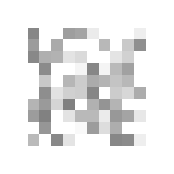
\begin{tikzpicture}[scale=0.15]
            \foreach \i in {0,...,99} {
                \pgfmathsetmacro\x{random(0,9)}
                \pgfmathsetmacro\y{random(0,9)}
                \pgfmathsetmacro\gray{random(0,100)}
                \fill[gray!\gray!white] (\x,\y) rectangle (\x+1,\y+1);
            }
        \end{tikzpicture}
    };
    
    % Flattened shuffled
    \draw[->, thick] (2,-5) -- (4,-5) node[midway, above] {Flatten};
    \node[draw, minimum width=0.5cm, minimum height=5cm] (vecshuf) at (5.5,-5) {};
    \node[right=0.2cm of vecshuf] {Same 3,072 values!};
    
    % MLP
    \node[draw, rounded corners, fill=red!20, minimum width=3cm, minimum height=1.5cm] (mlp) at (9,-2.5) {MLP};
    \draw[->, thick] (vec) -- (mlp);
    \draw[->, thick] (vecshuf) -- (mlp);
    
    % Same output
    \node[right=1cm of mlp] {Same output!};
\end{tikzpicture}
\caption{MLPs treat ordered and shuffled pixels identically - spatial structure is lost}
\end{figure}

\begin{tcolorbox}[colback=red!5!white, colframe=red!50!black, title=The Fatal Flaw]
An MLP treats an image as a ``bag of pixels'' with no spatial relationships. Whether the pixels are:
\begin{itemize}
    \item Arranged in their original 2D grid
    \item Randomly shuffled
    \item Sorted by intensity
\end{itemize}
The MLP produces the \textbf{same output} because it only sees a flat vector of numbers!
\end{tcolorbox}

\paragraph{Why This Matters for Generalization?}

This pixel-shuffling invariance reveals why MLPs struggle with image recognition:

\begin{enumerate}
    \item \textbf{No Feature Learning}: MLPs learn arbitrary patterns in the training data rather than meaningful visual features
    \item \textbf{Poor Generalization}: A slightly shifted object looks completely different as a flat vector
    \item \textbf{Inefficient Learning}: Must learn the same pattern separately at every possible position
\end{enumerate}

Empirically, a standard MLP achieves only $\approx 74\%$ accuracy on CIFAR-10, while humans easily reach $>99\%$.





If you do it for MNIST, however, the MLP's high accuracy on images is misleading. It doesn't learn what an object is truly made of, like the lines and curves that form a "3". Instead, it learns a single, rigid pattern—or "template"—for the entire image. This lack of structural understanding is why it can be easily fooled, often confidently identifying a "3" in an image of pure random static. This approach is brittle and only works when new images look almost exactly like the training examples. This fundamental failure shows why a different type of network is needed for vision: one designed from the ground up to recognize smaller, local features like edges and corners.


The reason humans are able to see is because our brains have a vast amount of knowledge about the world built into their structure. Similarly, the only reason CNNs can ``see'' is because a human has hard-coded the assumptions of \textbf{spatial locality} and \textbf{translation invariance} into the network's architecture via the cross-correlation operation. The network doesn't need to learn these fundamental properties of the visual world from data; it is given this knowledge from the start, allowing it to efficiently learn the meaningful patterns required for computer vision.


\section{The Solution: Exploiting Spatial Structure}

\subsection{Two Key Principles}

To overcome these limitations, we need to incorporate two fundamental properties of visual data:

\begin{principle}[Spatial Locality]
Nearby pixels are more related than distant ones. Edges, textures, and patterns emerge from \textbf{local neighborhoods}, not global pixel arrangements.
\end{principle}

\begin{principle}[Translation Equivariance]
The same feature detector should work regardless of position. A cat's ear is a cat's ear whether it appears in the top-left or bottom-right.
\end{principle}

\begin{figure}[h]
\centering
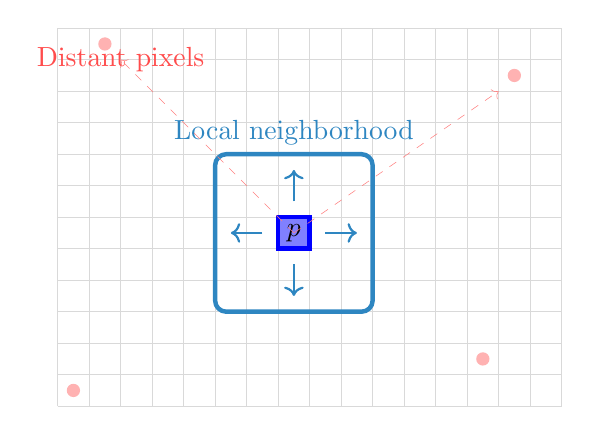
\begin{tikzpicture}[scale=0.8]
    % Grid representing image
    \draw[step=0.5, gray!30] (0,0) grid (8,6);
    
    % Center pixel
    \filldraw[fill=blue!50, draw=blue, ultra thick] (3.5,2.5) rectangle (4,3);
    \node at (3.75,2.75) {$p$};
    
    % Local neighborhood
    \draw[ultra thick, locality, rounded corners] (2.5,1.5) rectangle (5,4);
    \node[locality, above] at (3.75,4) {Local neighborhood};
    
    % Distant pixels
    \foreach \x/\y in {0.25/0.25, 7.25/5.25, 0.75/5.75, 6.75/0.75} {
        \fill[red!30] (\x,\y) circle (3pt);
    }
    \node[red!70] at (1,5.5) {Distant pixels};
    
    % Arrows showing influence
    \draw[->, thick, locality] (3.25,2.75) -- (2.75,2.75);
    \draw[->, thick, locality] (4.25,2.75) -- (4.75,2.75);
    \draw[->, thick, locality] (3.75,2.25) -- (3.75,1.75);
    \draw[->, thick, locality] (3.75,3.25) -- (3.75,3.75);
    
    \draw[->, very thin, dashed, red!50] (3.75,2.75) -- (1,5.5);
    \draw[->, very thin, dashed, red!50] (3.75,2.75) -- (7,5);
\end{tikzpicture}
\caption{Spatial locality: features depend on local neighborhoods}
\end{figure}



This suggests a new strategy: instead of one massive network looking at the entire image, what if we used a very small neural network to analyze one small patch at a time? This small network would act as a \textbf{feature detector}, and we could slide it across the entire image to find that feature everywhere.

To understand what these feature detectors do, let's first look at how computer vision experts used to design them by hand.






\subsection{Limitations of Hand-Crafted Kernels}
While these predefined kernels are interpretable, they have significant limitations:
\begin{enumerate}
    \item \textbf{Limited Expressiveness:} They can only detect simple, predefined patterns. They cannot capture complex features like ``cat ears" or ``car wheels."
    \item \textbf{Manual Feature Engineering:} Determining which kernels to use and how to combine them requires extensive domain expertise and experimentation.
    \item \textbf{No Adaptation:} Fixed kernels cannot adapt to the specific characteristics of a dataset. Kernels that work for one task may fail for another.
\end{enumerate}
The dream would be to have a system that could \textit{learn} the best kernels for a given task automatically. To understand how that's possible, we must first generalize the operation that these kernels perform.





\section{The Sliding Window Operation}

Before diving into neural networks, let's understand the core operation through a familiar example: smoothing noisy data.

\paragraph{Moving Average as Local Operation:}

A moving average implements locality with \emph{uniform} weights:

\begin{figure}[h]
\centering
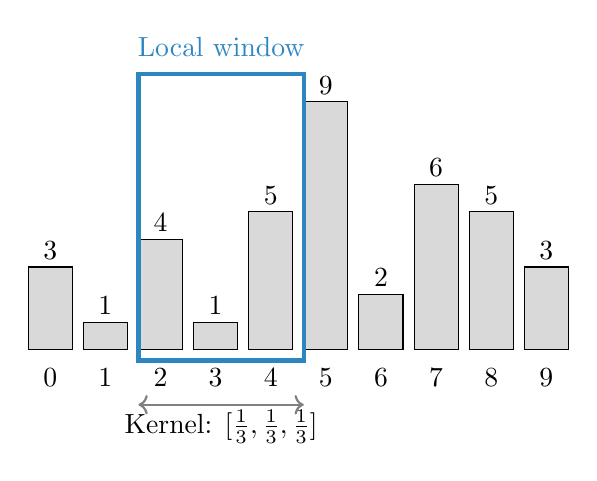
\begin{tikzpicture}[scale=0.7]
    % Signal values
    \foreach \i/\val in {0/3, 1/1, 2/4, 3/1, 4/5, 5/9, 6/2, 7/6, 8/5, 9/3} {
        \draw[fill=gray!30] (\i,0) rectangle (\i+0.8,\val*0.5);
        \node at (\i+0.4,-0.5) {\i};
        \node at (\i+0.4,\val*0.5+0.3) {\val};
    }
    
    % Local window
    \draw[ultra thick, locality] (2,-0.2) rectangle (5,5);
    \node[locality] at (3.5,5.5) {Local window};
    
    % Kernel weights visualization
    \node at (3.5,-1.4) {Kernel: $[\frac{1}{3}, \frac{1}{3}, \frac{1}{3}]$};
    % Show locality principle
    \draw[<->, thick, gray] (2,-1) -- (5,-1);
\end{tikzpicture}
\caption{Moving average: the simplest implementation of spatial locality}
\end{figure}


\paragraph{From 1D to 2D: Image Blurring}

A blur is essentially a \textbf{moving average} applied to the image's pixels. The process works as follows:
\begin{enumerate}
    \item We define a small window, or \textbf{kernel}, containing weights. For a simple blur, all weights are positive and sum to 1.
    \item We place this kernel over a patch of the input image.
    \item We perform an element-wise multiplication between the kernel's weights and the corresponding pixel values in the patch.
    \item We sum up all the results to get a single new pixel value.
    \item We \textbf{slide the window} across the entire image, repeating this process for every location to create a new, blurred image.
\end{enumerate}
Each new pixel is a weighted average of its neighbors, which smooths out the image and reduces detail.

\subsection{Generalizing the Operation with Other Kernels}
This same ``sliding window" operation can achieve much more than blurring. By simply changing the values in the kernel, we can create different feature detectors:
\begin{itemize}
    \item \textbf{Edge Detection:} An edge detection kernel (like a Sobel filter) contains both positive and negative values that sum to zero. When this kernel slides over a flat, uniform region, the output is zero. However, when it slides over an edge—a sharp change in pixel values—the sum of products becomes large (either positive or negative), thus highlighting the edge.
    \item \textbf{Sharpening:} A sharpening kernel amplifies the difference between a pixel and its neighbors, making edges and details more pronounced.
\end{itemize}
The mechanism is identical in all cases: a small kernel slides across the image, computing a sum of products at each location. The specific effect is determined entirely by the values within the kernel. We will drop the discussion of predetermined kernels here, but if interested, check out Appendix \ref{app:CV} for more on predetermined kernels and extensions.

\subsection{Naming the Operation: Cross-Correlation}
This powerful sliding window mechanism, where we compute a sum of element-wise products between a kernel and an image patch, is known as \textbf{cross-correlation}.

Mathematically, the 2D cross-correlation is defined as:
$$[H]_{i,j}=\sum_{a=-\Delta}^{\Delta}\sum_{b=-\Delta}^{\Delta}[V]_{a,b}[X]_{i+a,j+b}$$
Here, $V$ is the kernel, $X$ is the input image patch, and $H$ is the output feature map.

In the deep learning community, this operation is ubiquitously called a \textbf{convolution}. In pure mathematics, a true convolution involves flipping the kernel first. However, since the kernel's values are learned parameters, this distinction is inconsequential in practice, and the community uses the term ``convolution".


\begin{tcolorbox}[colback=blue!5!white, colframe=blue!50!black, title=Matrix View (Preview)]
When we ``slide a kernel,'' we're actually doing matrix multiplication with a special structure:
\begin{itemize}
    \item Each output is a dot product between kernel and input patch
    \item The matrix has repeated values along diagonals
    \item This structure enables massive parameter sharing
\end{itemize}
\end{tcolorbox}







\newpage
\section{The Leap to Learning: What if We Learn the Kernels?}

\subsection{From Hand-Crafted to Learned}

Computer vision experts spent decades designing kernels for specific features. But what if we could \textbf{learn} the optimal kernels automatically?

\begin{figure}[h]
\centering
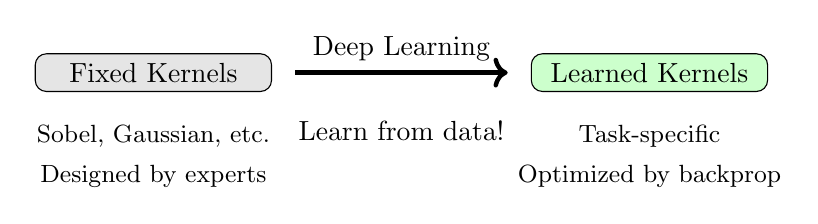
\begin{tikzpicture}[scale=0.9]
    % Fixed filters
    \node[draw, rounded corners, fill=gray!20, minimum width=3cm] (fixed) at (0,0) {Fixed Kernels};
    \node[below=0.3cm of fixed, font=\small] {Sobel, Gaussian, etc.};
    \node[below=0.8cm of fixed, font=\small] {Designed by experts};
    
    % Arrow
    \draw[->, ultra thick] (2,0) -- (5,0) node[midway, above] {Deep Learning};
    \node[below=0.5cm] at (3.5,0) {Learn from data!};
    
    % Learned filters
    \node[draw, rounded corners, fill=green!20, minimum width=3cm] (learned) at (7,0) {Learned Kernels};
    \node[below=0.3cm of learned, font=\small] {Task-specific};
    \node[below=0.8cm of learned, font=\small] {Optimized by backprop};
\end{tikzpicture}
\caption{The paradigm shift: from manual design to learning from data}
\end{figure}





Convolution has a crucial property that makes it perfect for images:

\begin{theorem}[Translation Equivariance]
If you shift the input, the output shifts by the same amount:
\[
\text{Conv}(\text{Shift}(X)) = \text{Shift}(\text{Conv}(X))
\]
\end{theorem}

\begin{figure}[h]
\centering
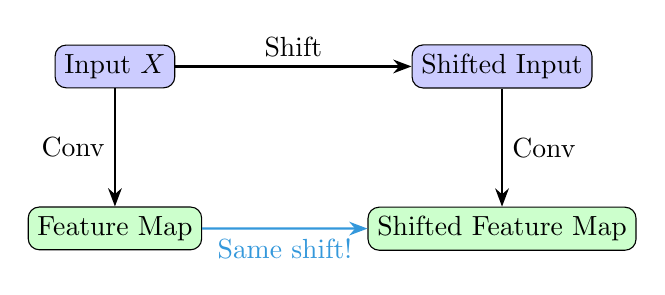
\begin{tikzpicture}[node distance=2cm, >=Stealth]
    % Nodes
    \node[draw, rounded corners, fill=blue!20] (x) {Input $X$};
    \node[draw, rounded corners, fill=blue!20, right=3cm of x] (xshift) {Shifted Input};
    \node[draw, rounded corners, fill=green!20, below=1.5cm of x] (y) {Feature Map};
    \node[draw, rounded corners, fill=green!20, below=1.5cm of xshift] (yshift) {Shifted Feature Map};
    
    % Arrows
    \draw[->, thick] (x) -- node[left] {Conv} (y);
    \draw[->, thick] (xshift) -- node[right] {Conv} (yshift);
    \draw[->, thick] (x) -- node[above] {Shift} (xshift);
    \draw[->, thick, equivariance] (y) -- node[below] {Same shift!} (yshift);
\end{tikzpicture}
\caption{Translation equivariance: features move with the input}
\end{figure}

This means:
\begin{itemize}
    \item The same kernel works everywhere in the image
    \item Features are detected regardless of position
    \item We only need to learn one detector, not thousands
\end{itemize}






\begin{tcolorbox}[colback=green!5!white, colframe=green!50!black, title=The Power of Equivariance]
Translation equivariance means:
\begin{itemize}
    \item Features are detected \emph{regardless of position}
    \item The same kernel works everywhere in the image
    \item We can share weights across all positions (parameter efficiency!)
    \item Feature maps preserve spatial relationships
\end{itemize}
\end{tcolorbox}

\begin{tcolorbox}[colback=purple!5!white, colframe=purple!50!black, title=Computational Magic (Preview)]
The equivariance property has a stunning consequence:
\begin{itemize}
    \item Convolution in space = Multiplication in frequency domain
    \item This enables FFT speedup: $O(n^2) \rightarrow O(n \log n)$
    \item The Fourier basis diagonalizes all translation-equivariant operators!
\end{itemize}
If interested, see Appendix \ref{app:circulant} for the mathematical beauty behind this.
\end{tcolorbox}



% \begin{tcolorbox}[colback=blue!5!white, colframe=blue!50!black, title=Learning Objectives]
% In this lecture, we will build upon our understanding of convolution to explore how modern CNNs are constructed. We will cover:
% \begin{itemize}
%     \item The core operations of a convolutional layer: \textbf{channels}, \textbf{padding}, and \textbf{strides}.
%     \item The role of \textbf{pooling} in creating invariance.
%     \item The architectural evolution from early networks like \textbf{LeNet} to modern powerhouses.
%     \item Key innovations like \textbf{1x1 convolutions}, \textbf{residual connections}, and network-in-network designs that enable deeper and more efficient models.
% \end{itemize}
% \end{tcolorbox}

\section{The Building Blocks of a Convolutional Layer}

In the last lecture, we established that the core of a CNN is the convolution operation, which applies a sliding, learnable filter (kernel) over an image. Now, let's refine that picture by introducing the essential components that give us full control over our network architecture.

\subsection{Padding: Preserving Spatial Dimensions}

When we convolve a kernel (e.g., 3×3) over an image, the output feature map is slightly smaller than the input image. This is because the kernel cannot be centered on the pixels at the very edge. If we stack many convolutional layers, our feature maps would shrink until they disappear entirely, limiting the depth of our network.

To avoid losing spatial extent at the borders and preserve the input size when desired, which keeps information about edge pixels and stride (the step size of the kernel) to control the output spatial resolution—for stride $>1$ the feature map shrinks, reducing computation and inducing sparsity in receptive fields


\begin{figure}[h]
\centering
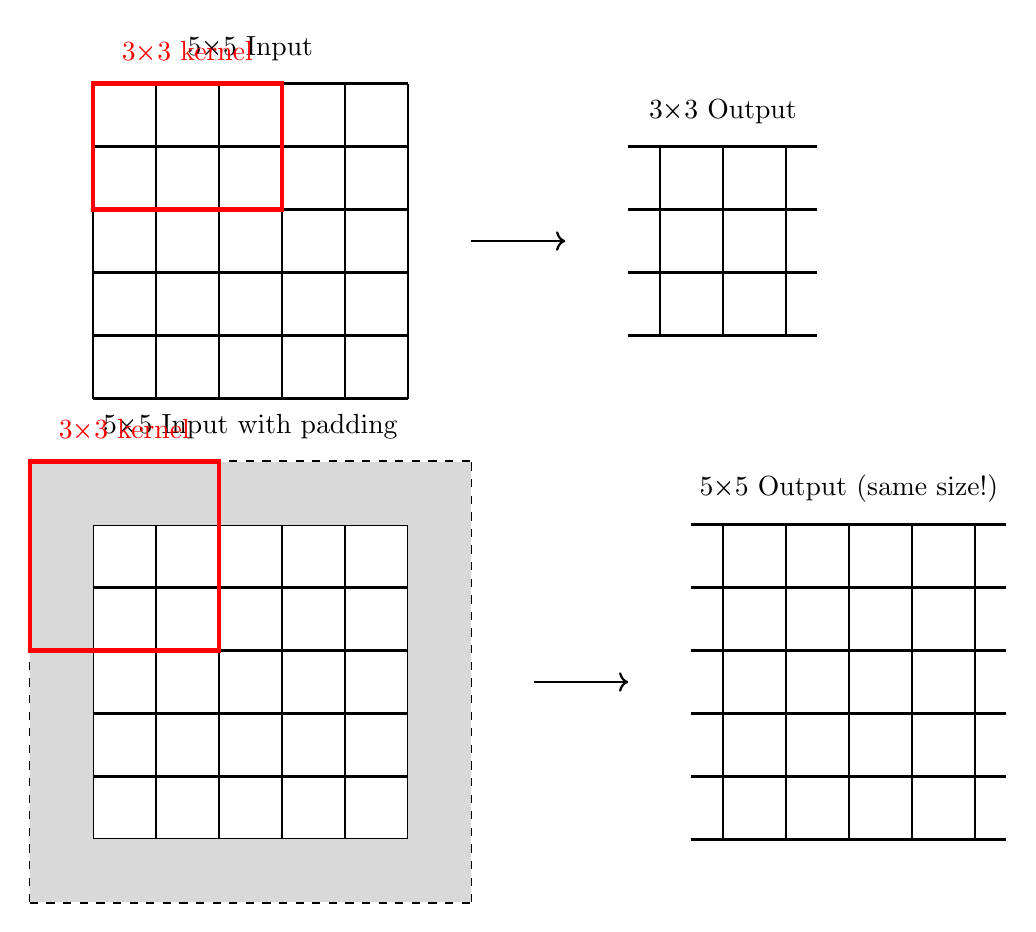
\begin{tikzpicture}[scale=0.8]
    % Input without padding
    \draw[thick] (0,0) grid (5,5);
    \node[above] at (2.5,5.2) {5×5 Input};
    
    % Kernel
    \draw[ultra thick, red] (0,3) rectangle (3,5);
    \node[red] at (1.5,5.5) {3×3 kernel};
    
    % Arrow
    \draw[->, thick] (6,2.5) -- (7.5,2.5);
    
    % Output
    \draw[thick] (8.5,1) grid (11.5,4);
    \node[above] at (10,4.2) {3×3 Output};
    
    % With padding
    \begin{scope}[yshift=-7cm]
        % Padded input
        \draw[thick, dashed] (-1,-1) grid (6,6);
        \draw[thick] (0,0) grid (5,5);
        \fill[gray!30] (-1,-1) rectangle (0,6);
        \fill[gray!30] (5,-1) rectangle (6,6);
        \fill[gray!30] (0,-1) rectangle (5,0);
        \fill[gray!30] (0,5) rectangle (5,6);
        \node[above] at (2.5,6.2) {5×5 Input with padding};
        
        % Kernel
        \draw[ultra thick, red] (-1,3) rectangle (2,6);
        \node[red] at (0.5,6.5) {3×3 kernel};
        
        % Arrow
        \draw[->, thick] (7,2.5) -- (8.5,2.5);
        
        % Output
        \draw[thick] (9.5,0) grid (14.5,5);
        \node[above] at (12,5.2) {5×5 Output (same size!)};
    \end{scope}
\end{tikzpicture}
\caption{Padding preserves spatial dimensions: top shows convolution without padding (output shrinks), bottom shows with padding (output size preserved).}
\end{figure}

The solution is simple: padding. We add a border of extra pixels (usually zeros) around the input image. For a 3×3 kernel, adding a 1-pixel border allows the output feature map to have the exact same height and width as the original input.

\begin{principle}[Padding]
Padding decouples the convolutional operation from spatial downsampling, allowing us to build arbitrarily deep networks without losing resolution at each layer.
\end{principle}

% Omitted from the public source snapshot: textbook-derived code removed to keep the
% book's independently licensed implementation boundary clear. See sources/README.md.

\subsection{Strides: Controlled Downsampling}

While we don't want to lose resolution unintentionally, we often want to \textit{deliberately} downsample the feature map. This reduces the computational load and helps the network learn more abstract features. We achieve this with strides.

A stride dictates the step size of the sliding kernel. A stride of 1 moves the kernel one pixel at a time. A stride of 2 skips every other pixel, effectively halving the height and width of the output feature map.

\begin{figure}[h]
\centering
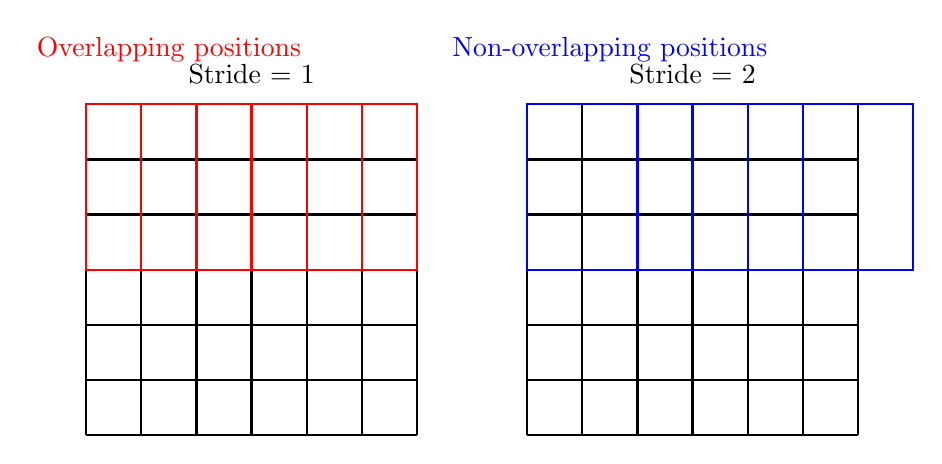
\begin{tikzpicture}[scale=0.7]
    % Stride 1
    \begin{scope}
        \draw[thick] (0,0) grid (6,6);
        \node[above] at (3,6.2) {Stride = 1};
        
        % Show kernel positions
        \foreach \x in {0,1,2,3} {
            \draw[red, thick] (\x,3) rectangle (\x+3,6);
        }
        \node[red] at (1.5,7) {Overlapping positions};
    \end{scope}
    
    % Stride 2
    \begin{scope}[xshift=8cm]
        \draw[thick] (0,0) grid (6,6);
        \node[above] at (3,6.2) {Stride = 2};
        
        % Show kernel positions
        \foreach \x in {0,2,4} {
            \draw[blue, thick] (\x,3) rectangle (\x+3,6);
        }
        \node[blue] at (1.5,7) {Non-overlapping positions};
    \end{scope}
\end{tikzpicture}
\caption{Stride controls how the kernel moves: stride=1 has overlapping receptive fields, stride=2 skips positions for downsampling.}
\end{figure}

% Omitted from the public source snapshot: textbook-derived code removed to keep the
% book's independently licensed implementation boundary clear. See sources/README.md.

\subsection{Channels: From Pixels to Features}

Images are not single matrices; they have multiple channels (e.g., Red, Green, and Blue). A convolutional layer can process multiple input channels and produce multiple output channels.

\begin{figure}[h]
\centering
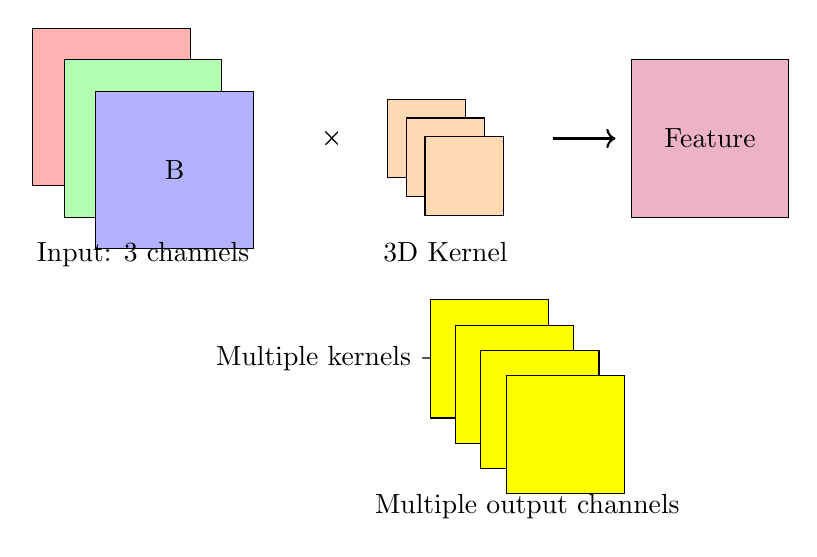
\begin{tikzpicture}[scale=0.8]
    % Input channels (RGB)
    \node[draw, minimum width=2cm, minimum height=2cm, fill=red!30] (r) at (0,0) {R};
    \node[draw, minimum width=2cm, minimum height=2cm, fill=green!30] (g) at (0.5,-0.5) {G};
    \node[draw, minimum width=2cm, minimum height=2cm, fill=blue!30] (b) at (1,-1) {B};
    \node[below] at (0.5,-2) {Input: 3 channels};
    
    % Kernels
    \node at (3.5,-0.5) {×};
    \foreach \i in {0,1,2} {
        \node[draw, minimum width=1cm, minimum height=1cm, fill=orange!30] at (5+\i*0.3,-0.5-\i*0.3) {};
    }
    \node[below] at (5.3,-2) {3D Kernel};
    
    % Arrow
    \draw[->, thick] (7,-0.5) -- (8,-0.5);
    
    % Single output channel
    \node[draw, minimum width=2cm, minimum height=2cm, fill=purple!30] at (9.5,-0.5) {Feature};
    
    % Multiple kernels
    \node at (3.5,-4) {Multiple kernels →};
    
    % Multiple output channels
    \foreach \i in {0,1,2,3} {
        \node[draw, minimum width=1.5cm, minimum height=1.5cm, fill=purple!\pgfmathresult!yellow] 
            at (6+\i*0.4,-4-\i*0.4) {};
    }
    \node[below] at (6.6,-6) {Multiple output channels};
\end{tikzpicture}
\caption{Channels in convolution: multiple input channels are processed by 3D kernels, and multiple kernels produce multiple output channels.}
\end{figure}

\begin{itemize}
    \item \textbf{Multiple Input Channels:} To process an RGB image, a convolutional kernel must also have a depth of 3. The 2D convolution becomes a 3D operation, where the weights for each channel are applied and the results are summed up to produce a single value in the output feature map.
    \item \textbf{Multiple Output Channels:} We can use multiple independent kernels in a single convolutional layer. Each kernel learns to detect a different feature (e.g., one kernel for vertical edges, another for green-red textures). The output of the layer is a stack of feature maps, one for each learned kernel.
\end{itemize}

% Omitted from the public source snapshot: D2L-derived code removed to keep the
% book's independently licensed implementation boundary clear. See sources/README.md.

\section{Pooling: Engineering Translation Invariance - From Features to Decisions}

\subsection{The Need for Invariance}
Think of a CNN's job in two parts. First, the convolution layers act like a \textbf{Feature Detective}. They scan the image for clues—a pointy ear, a whisker, a furry texture—and create a \textit{feature map} that shows exactly \textit{where} they found each clue. This property, where the map of clues shifts if the object shifts, is called \textbf{equivariance}. It's perfect for finding features.

However, the network's final job is to be a \textbf{Decision-Maker}. It must look at all the evidence and make a single judgment: ``Is this a cat?". For this final decision, it shouldn't matter if the cat was in the top-left or bottom-right corner. We need the final output to be the same regardless of the object's position. This property is called \textbf{invariance}.

The core challenge is bridging the gap from the detective's location-specific map to the judge's location-agnostic decision.

\begin{figure}[h]
\centering
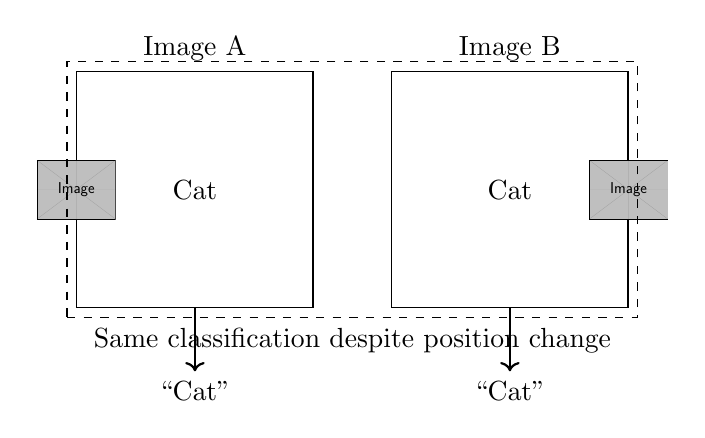
\begin{tikzpicture}[scale=0.8]
    % Two images with cat at different positions
    \node[draw, minimum width=3cm, minimum height=3cm, label=above:Image A] (imgA) at (0,0) {};
    \node at (imgA.west) {\includegraphics[width=1cm]{example-image}};
    \node at (imgA.center) {Cat};
    
    \node[draw, minimum width=3cm, minimum height=3cm, label=above:Image B] (imgB) at (5,0) {};
    \node at (imgB.east) {\includegraphics[width=1cm]{example-image}};
    \node at (imgB.center) {Cat};
    
    % Classification
    \draw[->, thick] (imgA.south) -- ++(0,-1) node[below] {``Cat''};
    \draw[->, thick] (imgB.south) -- ++(0,-1) node[below] {``Cat''};
    
    \node[draw, dashed, fit=(imgA)(imgB), label=below:Same classification despite position change] {};
\end{tikzpicture}
\caption{Classification requires position invariance}
\end{figure}

\subsection{Pooling: From Equivariance to Invariance}
The solution is \textbf{pooling}. Pooling builds the bridge from equivariance to invariance by \textbf{summarizing the evidence} in local neighborhoods. Instead of tracking the exact location of every clue, we condense the information, making the network less sensitive to precise positions.

This is done by sliding a window across the feature map and aggregating the values within it into a single value. This has two key benefits:
\begin{enumerate}
    \item It shrinks the size of the feature map, making the network more efficient.
    \item It creates \textbf{local translation invariance}. A small shift in a feature's position inside the pooling window often won't change the summarized output. By stacking these layers, the network becomes increasingly invariant to feature location.
\end{enumerate}

\begin{figure}[h]
\centering
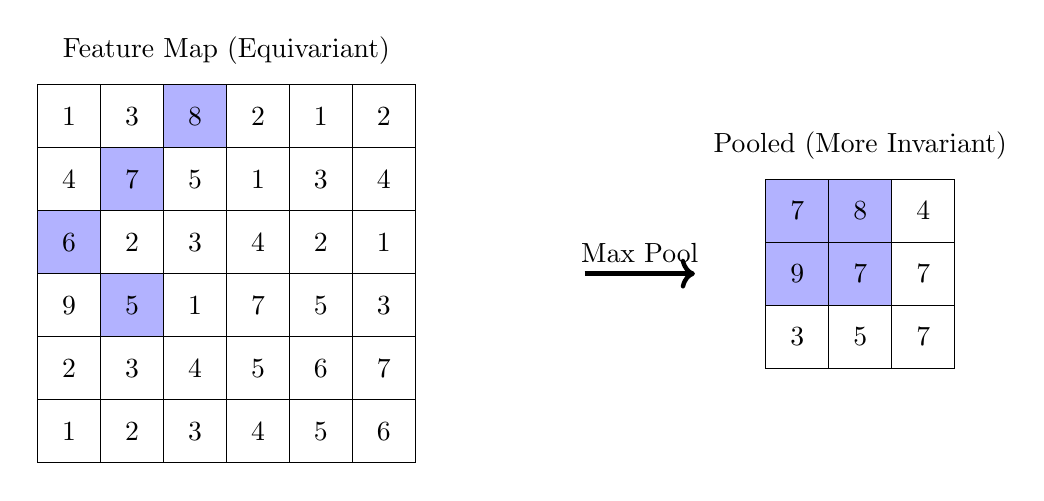
\begin{tikzpicture}[
    scale=0.7,
    featuremap/.style={matrix of nodes, nodes={draw, minimum size=8mm}, row sep=-\pgflinewidth, column sep=-\pgflinewidth}
]
    % Feature map
    \matrix[featuremap] (feat) at (0,0) {
        1 & 3 & |[fill=blue!30]| 8 & 2 & 1 & 2 \\
        4 & |[fill=blue!30]| 7 & 5 & 1 & 3 & 4 \\
        |[fill=blue!30]| 6 & 2 & 3 & 4 & 2 & 1 \\
        9 & |[fill=blue!30]| 5 & 1 & 7 & 5 & 3 \\
        2 & 3 & 4 & 5 & 6 & 7 \\
        1 & 2 & 3 & 4 & 5 & 6 \\
    };
    \node[above] at (feat.north) {Feature Map (Equivariant)};
    
    % Arrow
    \draw[->, ultra thick] (6.5,0) -- (8.5,0) node[midway, above] {Max Pool};
    
    % Pooled result
    \matrix[featuremap] (pool) at (11.5,0) {
        |[fill=blue!30]| 7 & |[fill=blue!30]| 8 & 4 \\
        |[fill=blue!30]| 9 & |[fill=blue!30]| 7 & 7 \\
        3 & 5 & 7 \\
    };
    \node[above] at (pool.north) {Pooled (More Invariant)};

\end{tikzpicture}
\caption{Pooling provides local translation invariance by summarizing neighborhoods.}
\end{figure}

\subsection{Types of Pooling and Their Properties}
There are two main strategies for summarizing the evidence in a neighborhood:

\begin{itemize}
    \item \textbf{Max Pooling (Finding the Strongest Clue):} This is the most common approach. For each neighborhood, we ask: \textit{``What's the strongest piece of evidence here?"} We take only the \textbf{maximum} activation value and discard the rest. This method excels at preserving the sharpest, most important features the detective found.

    \item \textbf{Average Pooling (Getting the General Vibe):} For each neighborhood, we ask: \textit{``What's the \textbf{average} level of evidence here?"} This gives a smoother, more general summary of the features in the region but can sometimes dilute the strength of one critical clue.
\end{itemize}

Ultimately, both methods help the network transition from finding features to making a final, robust classification based on \textit{what} features are present, not \textit{where} they are located.

\begin{figure}[ht]
\centering
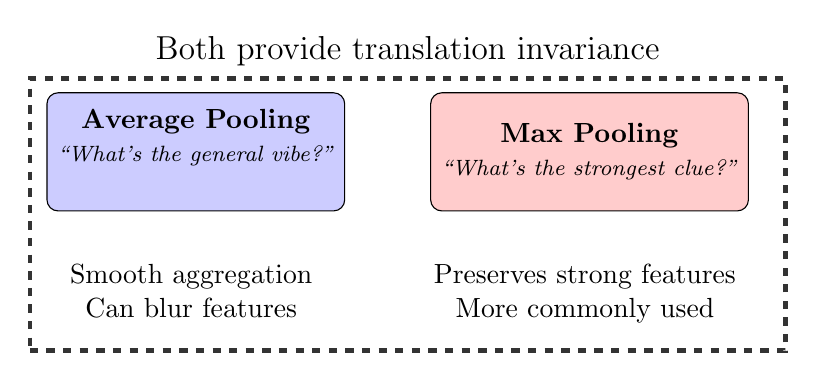
\begin{tikzpicture}[
    every node/.style={align=center},
    node distance=1cm
]
    % Average pooling
    \node[draw, rounded corners, fill=blue!20, minimum width=3.5cm, minimum height=1.5cm] (avg) at (0,0) {
        \textbf{Average Pooling}\\
        \footnotesize \textit{``What's the general vibe?"}\\
    };
    
    % Max pooling
    \node[draw, rounded corners, fill=red!20, minimum width=3.5cm, minimum height=1.5cm] (max) at (5,0) {
        \textbf{Max Pooling}\\
        \footnotesize \textit{``What's the strongest clue?"}
    };
    
    % Properties
    \node[below=0.5cm of avg] (avgProp) {
        \begin{tabular}{c}
        Smooth aggregation\\
        Can blur features
        \end{tabular}
    };
    
    \node[below=0.5cm of max] (maxProp) {
        \begin{tabular}{c}
        Preserves strong features\\
        More commonly used
        \end{tabular}
    };
    
    % Both achieve invariance
    \node[draw=black!80, dashed, ultra thick, 
          fit={(avg) (max) (avgProp) (maxProp)}, 
          inner sep=5pt,
          label={[font=\large]above:Both provide translation invariance}] {};
\end{tikzpicture}
\caption{Comparison of pooling operations in CNNs}
\label{fig:pooling_comparison}
\end{figure}








As we discussed, convolution is equivariant. To achieve the invariance needed for classification, we introduce pooling layers. A pooling layer aggressively downsamples the feature map by taking a summary of a local neighborhood.

% Omitted from the public source snapshot: textbook-derived code removed to keep the
% book's independently licensed implementation boundary clear. See sources/README.md.

By taking the max or average, the network becomes less sensitive to the exact location of a feature within the pooling window. Modern networks heavily favor max pooling over average pooling, as it preserves the strongest feature activations.





\begin{figure}[h]
\centering
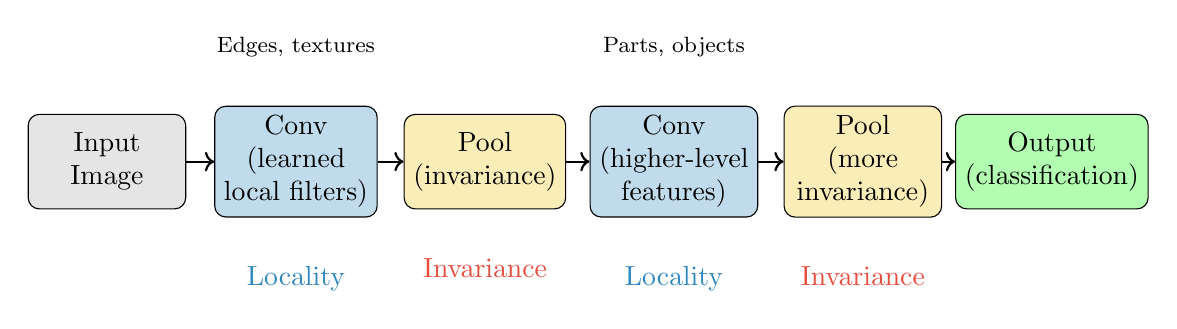
\begin{tikzpicture}[scale=0.8, 
    layer/.style={rectangle, draw, rounded corners, minimum width=2cm, minimum height=1.2cm, align=center},
    pool/.style={layer, fill=pooling!30}
]
    % Architecture
    \node[layer, fill=gray!20] (input) at (0,0) {Input\\Image};
    
    \node[layer, fill=locality!30] (conv1) at (3,0) {Conv\\(learned\\local filters)};
    \node[pool] (pool1) at (6,0) {Pool\\(invariance)};
    
    \node[layer, fill=locality!30] (conv2) at (9,0) {Conv\\(higher-level\\features)};
    \node[pool] (pool2) at (12,0) {Pool\\(more\\invariance)};
    
    \node[layer, fill=green!30] (output) at (15,0) {Output\\(classification)};
    
    % Connections
    \draw[->, thick] (input) -- (conv1);
    \draw[->, thick] (conv1) -- (pool1);
    \draw[->, thick] (pool1) -- (conv2);
    \draw[->, thick] (conv2) -- (pool2);
    \draw[->, thick] (pool2) -- (output);
    
    % Principles
    \node[below=0.5cm of conv1, locality] {Locality};
    \node[below=0.5cm of pool1, invariance] {Invariance};
    \node[below=0.5cm of conv2, locality] {Locality};
    \node[below=0.5cm of pool2, invariance] {Invariance};
    
    % What's learned
    \node[above=0.5cm of conv1] {\footnotesize Edges, textures};
    \node[above=0.5cm of conv2] {\footnotesize Parts, objects};
\end{tikzpicture}
\caption{CNN architecture: alternating locality (conv) and invariance (pool)}
\end{figure}



\section{Evolution of CNN Architectures}

The history of CNNs is a story of combining these building blocks in ever-deeper and more clever ways, driven by increases in data and computational power.

% ##### INSERT THIS CODE INTO YOUR .TEX FILE #####
% Recommended location: After ``\section{Evolution of CNN Architectures}" and
% before ``\subsection{LeNet-5 (1998): The Pioneer}"

\subsection{Reusing Learned Features: The Power of Transfer Learning}

We've established that the convolutional layers of a CNN learn to be powerful, hierarchical feature extractors. Early layers learn generic features like edges and color gradients, while deeper layers learn more complex and abstract features like textures, patterns, and object parts (e.g., eyes, wheels, leaves).

This raises a powerful question: are the features learned for one task useful for another? For instance, if a network is trained on the massive ImageNet dataset (with 1,000 classes like ``dog", ``car", ``chair"), its learned ability to detect edges, textures, shapes, and object parts seems universally useful for almost any visual task.

This is the core idea behind \textbf{transfer learning}: we can reuse a network trained on a very large dataset as a feature extractor for a new, different task, especially one where we have limited data.

\begin{tcolorbox}[colback=blue!5!white, colframe=blue!50!black, title=The Transfer Learning Recipe]
The process is conceptually simple and incredibly effective:
\begin{enumerate}
    \item \textbf{Take a pre-trained network:} Start with a state-of-the-art CNN (like VGG, ResNet, or EfficientNet) that has already been trained on a large benchmark dataset like ImageNet.
    \item \textbf{Split the model:} A CNN is composed of two parts: the \textbf{convolutional base} (the stack of conv/pool layers that acts as a feature extractor) and the \textbf{classifier head} (the final fully-connected layers that make the classification decision).
    \item \textbf{Freeze the base:} We keep the convolutional base and lock its weights. We assume it's already a great general-purpose feature extractor.
    \item \textbf{Replace the head:} We discard the original classifier (which was trained for 1,000 ImageNet classes) and attach a new, smaller classifier tailored to our specific task (e.g., classifying between ``healthy" and ``diseased" plant leaves).
    \item \textbf{Train on the new task:} We then train \textit{only} the new classifier layers on our smaller, custom dataset. Since the vast majority of the network's parameters are frozen, this training is very fast and requires much less data.
\end{enumerate}
\end{tcolorbox}

\begin{figure}[h!]
\centering
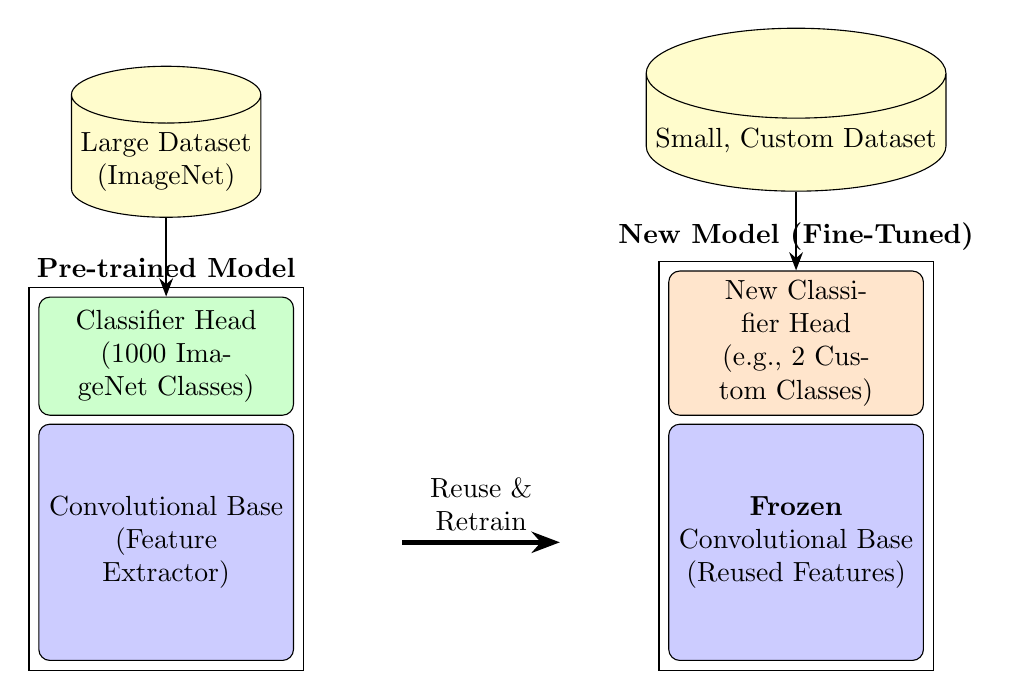
\begin{tikzpicture}[
    node distance=1cm,
    block/.style={rectangle, draw, rounded corners, fill=gray!10, text width=3cm, minimum height=1.5cm, align=center},
    convbase/.style={block, fill=blue!20, minimum height=3cm},
    classifier/.style={block, fill=green!20, text width=3cm},
    dataset/.style={cylinder, shape border rotate=90, draw, fill=yellow!20, aspect=0.3, minimum height=1.5cm, align=center},
    arrow/.style={->, >=Stealth, thick}
]
    % Left side: Pre-trained Model
    \node[convbase] (base) {Convolutional Base \\ (Feature Extractor)};
    \node[classifier, above=0.1cm of base] (head) {Classifier Head \\ (1000 ImageNet Classes)};
    \node[dataset, above=1cm of head] (imagenet) {Large Dataset \\ (ImageNet)};
    \draw[arrow] (imagenet) -- (head);
    \node[draw, fit=(base)(head), label={[font=\bfseries]above:Pre-trained Model}] {};

    % Arrow in the middle
    \draw[arrow, ultra thick] (3,0) -- (5,0) node[midway, above, align=center] {Reuse \& \\ Retrain};

    % Right side: New Model
    \begin{scope}[xshift=8cm]
        \node[convbase] (newbase) {\textbf{Frozen} \\ Convolutional Base \\ (Reused Features)};
        \node[classifier, fill=orange!20, above=0.1cm of newbase] (newhead) {New Classifier Head \\ (e.g., 2 Custom Classes)};
        \node[dataset, above=1cm of newhead] (newdata) {Small, Custom Dataset};
        \draw[arrow] (newdata) -- (newhead);
        \node[draw, fit=(newbase)(newhead), label={[font=\bfseries]above:New Model (Fine-Tuned)}] {};
    \end{scope}
\end{tikzpicture}
\caption{The transfer learning workflow: The powerful feature extractor from a model trained on a large dataset is frozen and repurposed with a new classifier head, which is then trained on a smaller, specific dataset.}
\label{fig:transfer_learning}
\end{figure}

Transfer learning is one of the most significant reasons for the widespread success of deep learning in computer vision. It allows practitioners with limited data and computational resources to achieve state-of-the-art results by standing on the shoulders of giants. As we explore famous architectures, keep in mind that their primary modern use is often as a foundation for transfer learning.


\subsection{LeNet-5 (1998): The Pioneer}

LeNet-5 was designed to read handwritten digits. Its architecture became the template for all that followed:

% Omitted from the public source snapshot: textbook-derived architecture code removed
% to keep the book's independently licensed implementation boundary clear.

\begin{figure}[ht]
\centering
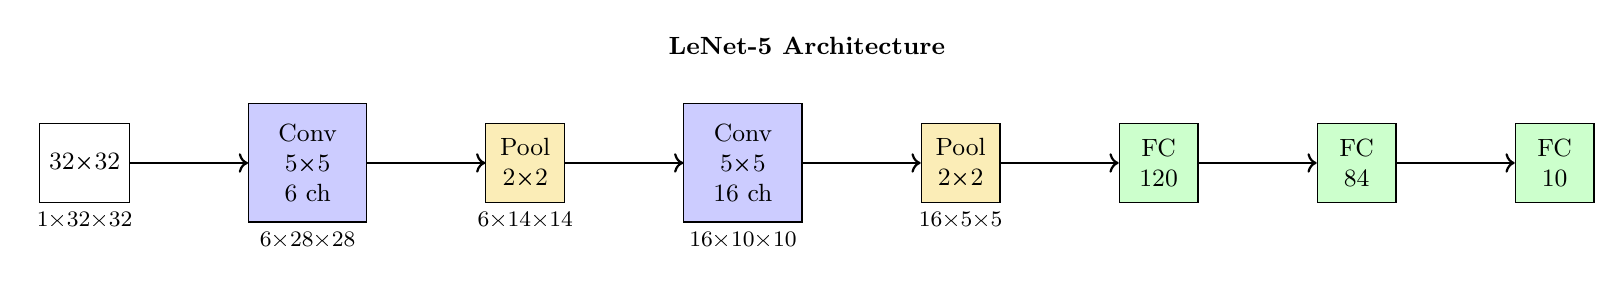
\begin{tikzpicture}[
    scale=0.4,
    node distance=1.5cm,
    every node/.style={font=\small, align=center},
    conv/.style={draw, minimum width=1.5cm, minimum height=1.5cm, fill=blue!20},
    pool/.style={draw, minimum width=1cm, minimum height=1cm, fill=pooling!30},
    fc/.style={draw, minimum width=1cm, minimum height=1cm, fill=green!20},
    dim/.style={below, font=\footnotesize}
]
    % Input
    \node[draw, minimum width=1cm, minimum height=1cm] (input) {32×32};
    \node[dim] at (input.south) {1×32×32};
    
    % Conv1
    \node[conv, right=of input] (conv1) {Conv\\5×5\\6 ch};
    \node[dim] at (conv1.south) {6×28×28};
    
    % Pool1
    \node[pool, right=of conv1] (pool1) {Pool\\2×2};
    \node[dim] at (pool1.south) {6×14×14};
    
    % Conv2
    \node[conv, right=of pool1] (conv2) {Conv\\5×5\\16 ch};
    \node[dim] at (conv2.south) {16×10×10};
    
    % Pool2
    \node[pool, right=of conv2] (pool2) {Pool\\2×2};
    \node[dim] at (pool2.south) {16×5×5};
    
    % FC layers
    \node[fc, right=of pool2] (fc1) {FC\\120};
    \node[fc, right=of fc1] (fc2) {FC\\84};
    \node[fc, right=of fc2] (fc3) {FC\\10};
    
    % Connections
    \foreach \i/\j in {input/conv1, conv1/pool1, pool1/conv2, conv2/pool2, pool2/fc1, fc1/fc2, fc2/fc3} {
        \draw[->, thick] (\i) -- (\j);
    }
    
    % Architecture label
    \node[above=0.5cm of current bounding box.north] {
        \textbf{LeNet-5 Architecture}
    };
\end{tikzpicture}
\caption{LeNet-5 architecture showing the alternating pattern of convolutional and pooling layers, followed by fully connected layers. The dimensions below each layer show (channels × height × width).}
\label{fig:lenet_architecture}
\end{figure}

\subsection{AlexNet (2012): The Game Changer}

AlexNet won ImageNet by a massive margin. The key differences from LeNet were:

% Omitted from the public source snapshot: textbook-derived architecture code removed
% to keep the book's independently licensed implementation boundary clear.

Key innovations:
\begin{enumerate}
    \item \textbf{Scale:} Much deeper and wider to handle ImageNet complexity
    \item \textbf{ReLU Activation:} Replaced sigmoid, solving vanishing gradients
    \item \textbf{Max Pooling:} More aggressive feature selection than average pooling
    \item \textbf{Dropout:} Modern regularization technique
    \item \textbf{GPU Training:} Enabled by CUDA acceleration
\end{enumerate}

\section{Innovations in Modern CNNs}

\subsection{VGG: The Power of Simplicity and Depth}

VGG showed that using only 3×3 kernels throughout the network was more effective than larger kernels:

% Omitted from the public source snapshot: textbook-derived architecture code removed
% to keep the book's independently licensed implementation boundary clear.

\begin{tcolorbox}[colback=green!5!white, colframe=green!50!black, title=Why 3×3 Kernels?]
Two 3×3 convolutions have the same receptive field as one 5×5 convolution, but:
\begin{itemize}
    \item Use 18 parameters vs 25 (28\% fewer)
    \item Have two non-linearities instead of one
    \item Are easier to optimize
\end{itemize}
This principle now dominates modern architecture design.
\end{tcolorbox}

\subsection{Network in Network: 1×1 Convolutions}

The Network in Network (NiN) paper introduced two game-changing ideas:

% Omitted from the public source snapshot: textbook-derived architecture code removed
% to keep the book's independently licensed implementation boundary clear.

Key innovations:
\begin{enumerate}
    \item \textbf{1×1 Convolutions:} Act as channel-wise fully connected layers
    \item \textbf{Global Average Pooling:} Replaces huge FC layers, drastically reducing parameters
\end{enumerate}

\subsection{GoogLeNet/Inception: Multi-Scale Feature Extraction}

The Inception module processes input at multiple scales simultaneously:

% Omitted from the public source snapshot: textbook-derived architecture code removed
% to keep the book's independently licensed implementation boundary clear.

\subsection{ResNet: The Power of Residual Connections}

ResNet introduced skip connections that revolutionized deep learning:

% Omitted from the public source snapshot: textbook-derived architecture code removed
% to keep the book's independently licensed implementation boundary clear.

\begin{figure}[ht]
\centering
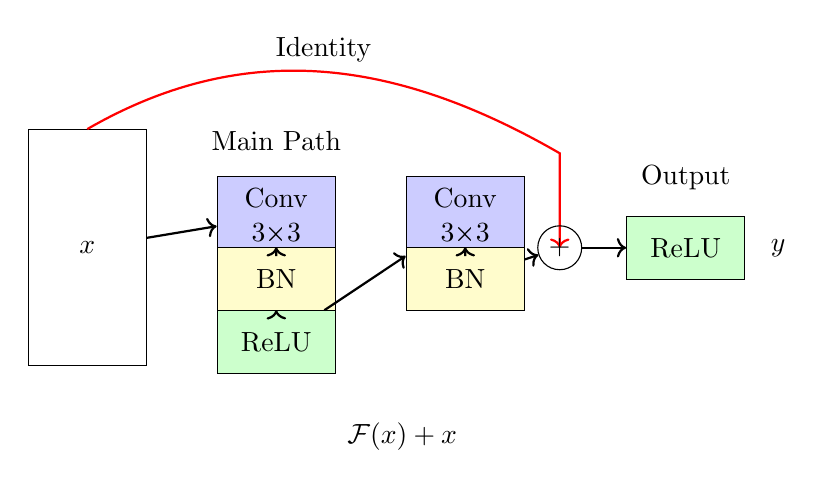
\begin{tikzpicture}[
    scale=0.8,
    every node/.style={align=center},
    conv/.style={draw, fill=blue!20, minimum width=1.5cm, minimum height=1cm},
    bn/.style={draw, fill=yellow!20, minimum width=1.5cm, minimum height=0.8cm},
    relu/.style={draw, fill=green!20, minimum width=1.5cm, minimum height=0.8cm},
    arrow/.style={->, thick}
]
    % Input
    \node[draw, minimum width=1.5cm, minimum height=3cm] (input) at (0,0) {$x$};
    
    % Main path
    \node[conv] (conv1) at (3,0.5) {Conv\\3×3};
    \node[bn] (bn1) at (3,-0.5) {BN};
    \node[relu] (relu1) at (3,-1.5) {ReLU};
    
    \node[conv] (conv2) at (6,0.5) {Conv\\3×3};
    \node[bn] (bn2) at (6,-0.5) {BN};
    
    % Skip connection
    \draw[arrow, red] (input.north) to[out=30,in=150] node[above, midway, black] {Identity} (7.5,1.5) -- (7.5,0);
    
    % Addition
    \node[draw, circle, inner sep=2pt] (add) at (7.5,0) {+};
    
    % Output
    \node[relu] (relu2) at (9.5,0) {ReLU};
    \node[right=0.2cm of relu2] {$y$};
    
    % Connections
    \foreach \i/\j in {input/conv1, conv1/bn1, bn1/relu1, relu1/conv2, conv2/bn2, bn2/add, add/relu2} {
        \draw[arrow] (\i) -- (\j);
    }
    
    % Formula
    \node at (5,-3) {$\mathcal{F}(x) + x$};
    
    % Labels
    \node[above=0.2cm of conv1] {Main Path};
    \node[above=0.2cm of relu2] {Output};
\end{tikzpicture}
\caption{Residual block architecture showing the skip connection that enables direct gradient flow. The identity connection allows the network to learn residual functions $\mathcal{F}(x) = y - x$ rather than direct transformations.}
\label{fig:residual_block}
\end{figure}

\section{Modern Efficiency Techniques}

\subsection{Depthwise Separable Convolutions}

MobileNet introduced depthwise separable convolutions for efficiency:

% Omitted from the public source snapshot: architecture code of uncertain provenance
% removed conservatively. See sources/README.md.

\section{Summary and Key Takeaways}

\begin{tcolorbox}[colback=green!5!white, colframe=green!50!black, title=Evolution of CNN Design]
\begin{enumerate}
    \item \textbf{LeNet (1998)}: Established the conv→pool→FC template
    \item \textbf{AlexNet (2012)}: Scaled up with ReLU, dropout, and GPUs
    \item \textbf{VGG (2014)}: Showed deep stacks of 3×3 convs beat larger kernels
    \item \textbf{NiN (2014)}: Introduced 1×1 convs and global average pooling
    \item \textbf{GoogLeNet (2014)}: Multi-scale processing with Inception modules
    \item \textbf{ResNet (2015)}: Skip connections enable training 100+ layer networks
    \item \textbf{MobileNet (2017)}: Efficient architectures for mobile deployment
\end{enumerate}
\end{tcolorbox}

\begin{tcolorbox}[colback=blue!5!white, colframe=blue!50!black, title=Design Principles]
Modern CNN design follows these principles:
\begin{itemize}
    \item \textbf{Deeper is better} - if you can train it (use residual connections)
    \item \textbf{3×3 kernels rule} - stack them for larger receptive fields
    \item \textbf{1×1 convolutions} - for channel mixing and dimensionality reduction
    \item \textbf{Replace FC with global pooling} - massive parameter reduction
    \item \textbf{Batch normalization} - for stable training
    \item \textbf{Depthwise separable} - for mobile/edge deployment
\end{itemize}
\end{tcolorbox}

\section{Exercises}

\subsection{Understanding the Building Blocks}
\begin{enumerate}
    \item Calculate the output size for a 32×32 input with: kernel=5×5, stride=2, padding=2
    \item Why does a 1×1 convolution still perform a meaningful operation?
    \item Implement a custom pooling operation that returns both max and average values
\end{enumerate}

\subsection{Architecture Analysis}
\begin{enumerate}
    \item Count the parameters in LeNet vs AlexNet. Where is the biggest difference?
    \item Prove that two 3×3 convolutions have the same receptive field as one 5×5
    \item Design a ``bottleneck" block that reduces computation using 1×1 convolutions
\end{enumerate}

\subsection{Implementation Challenges}
\begin{enumerate}
    \item Implement a simplified VGG-11 and train on CIFAR-10
    \item Add residual connections to VGG - does it improve training?
    \item Compare the speed and accuracy of standard vs depthwise separable convolutions
\end{enumerate}

\subsection{Modern Explorations}
\begin{enumerate}
    \item Research: How do Vision Transformers compare to CNNs?
    \item Implement grouped convolutions and compare to standard convolutions
    \item Design your own Inception-style module with different kernel sizes
\end{enumerate}

\section{Next Lecture Preview}

In the next lecture, we'll dive deep into training these architectures:
\begin{itemize}
    \item Data augmentation techniques
    \item Transfer learning and fine-tuning
    \item Practical training tips and tricks
    \item Building a complete image classification pipeline
\end{itemize}



\section{Why 3×3 Kernels Dominate}

\subsection{The Evolution of Kernel Sizes}

\begin{itemize}
    \item \textbf{AlexNet (2012)}: Used 11×11, 5×5, and 3×3 kernels
    \item \textbf{ZFNet (2013)}: Reduced to 7×7, showing cleaner learned patterns
    \item \textbf{VGG (2014)}: Revolutionary use of only 3×3 kernels
\end{itemize}

\subsection{The Efficiency Secret}

Two 3×3 convolutions have the same receptive field as one 5×5, but:
\begin{itemize}
    \item Parameters: $2 \times (3 \times 3) = 18$ vs $5 \times 5 = 25$ (28\% fewer!)
    \item More non-linearity: Two ReLU activations vs one
    \item Better gradient flow during training
\end{itemize}

\begin{figure}[h]
\centering
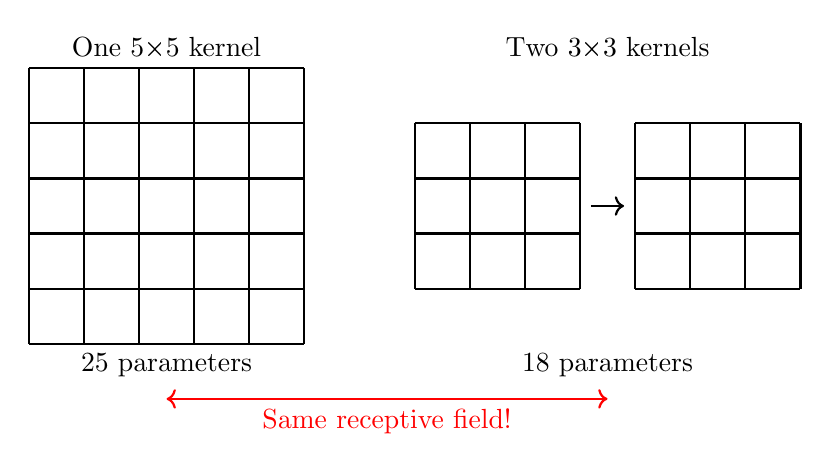
\begin{tikzpicture}[scale=0.7]
    % Single 5x5
    \draw[thick] (0,0) grid (5,5);
    \node[above] at (2.5,5) {One 5×5 kernel};
    \node[below] at (2.5,0) {25 parameters};
    
    % Two 3x3
    \draw[thick] (7,1) grid (10,4);
    \draw[thick] (11,1) grid (14,4);
    \draw[->, thick] (10.2,2.5) -- (10.8,2.5);
    \node[above] at (10.5,5) {Two 3×3 kernels};
    \node[below] at (10.5,0) {18 parameters};
    
    % Same receptive field
    \draw[<->, thick, red] (2.5,-1) -- (10.5,-1) node[midway, below] {Same receptive field!};
\end{tikzpicture}
\caption{Stacking small kernels is more efficient than one large kernel}
\end{figure}











\newpage
\appendix
\section{The Choice of Kernel Size: Why Everyone Loves 3×3}\label{app:3x3}

Now that we understand kernels can be learned automatically, a natural question arises: what size should these kernels be? The kernel size determines both the height and width of the filters and the size of the input patch we examine at each position. While we could theoretically choose any size from 1×1 up to the full input resolution, certain sizes have proven particularly effective.

\paragraph{A Brief History Through ImageNet}

The evolution of kernel size preferences tells an interesting story. In 2012, AlexNet became the first CNN to win the ImageNet competition. As a pioneer, it hadn't yet settled on what we now consider standard practices—it used an 11×11 kernel for its first convolution, 5×5 for the second, and 3×3 for the remaining layers.

The following year, Matt Zeiler won with an optimized version of AlexNet. One key optimization was reducing the first layer's kernel from 11×11 to 7×7. This led to cleaner filter patterns: the 11×11 kernels showed a mix of high and low frequency patterns with poor coverage of medium-sized features, while 7×7 kernels covered medium frequencies much better with more vivid low-frequency patterns.

In 2014, the Visual Geometry Group (VGG) from Oxford made a breakthrough by using exclusively 3×3 kernels throughout their network. They discovered something remarkable: \textbf{we don't need larger kernels}.

The key insight involves \textbf{receptive fields}. When we chain multiple 3×3 convolutions:
\begin{itemize}
    \item Each pixel in the first layer sees a 3×3 patch of the input
    \item The second layer sees a 3×3 patch of the first layer's output
    \item But that 3×3 patch in the first layer corresponds to a 5×5 area in the original input
    \item Therefore, two 3×3 convolutions have the same receptive field as one 5×5 convolution
\end{itemize}

\paragraph{The Efficiency Advantage}

This isn't just an interesting mathematical property—it provides significant computational benefits:
\begin{itemize}
    \item Two 3×3 convolutions use only \textbf{72\%} of the parameters and computation of a single 5×5
    \item Three 3×3 convolutions use only \textbf{55\%} of the resources of a single 7×7
\end{itemize}

The one exception is the very first layer. Since the input typically has only three channels (RGB), using a slightly larger kernel (5×5 or 7×7) can be more efficient for this initial feature extraction.

\paragraph{The Role of 1×1 Convolutions}

The other commonly used kernel size is 1×1. While it might seem strange to have a ``convolution'' that looks at only a single pixel, these serve an important purpose: they're the most efficient way to change the number of channels in your feature maps. They act like a fully connected layer applied independently at each spatial position, allowing the network to learn cross-channel interactions without any spatial mixing.

\paragraph{Why Not Even-Sized Kernels?}

Interestingly, even-sized kernels (2×2, 4×4, etc.) are virtually never used in practice. The asymmetry they introduce when determining the ``center'' of the kernel makes them awkward for maintaining spatial alignment through the network.

In summary, modern CNNs predominantly use 3×3 kernels for their optimal balance of expressiveness and efficiency, with 1×1 kernels for channel manipulation and occasionally larger kernels (5×5 or 7×7) for the first layer.




\section{Beyond Blurring: Feature Detection with Predetermind Kernels}\label{app:CV}

\paragraph{Edge Detection}

By changing the kernel values, we can detect features instead of blurring:

\begin{figure}[h]
\centering
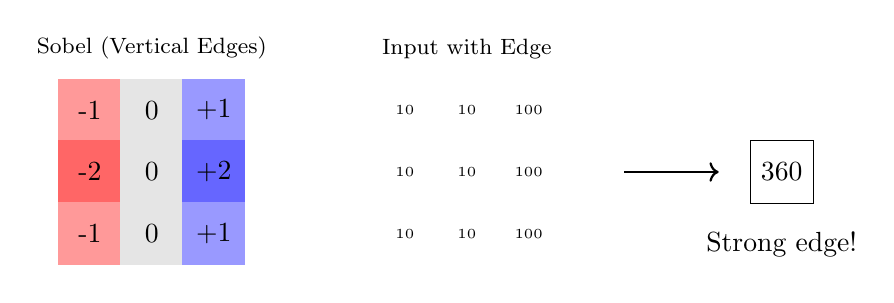
\begin{tikzpicture}[scale=0.8]
    % Sobel X kernel
    \matrix[matrix of nodes, nodes={minimum size=0.8cm, anchor=center}, 
            row sep=-\pgflinewidth, column sep=-\pgflinewidth,
            label={[font=\footnotesize]above:Sobel (Vertical Edges)}] (sobel) at (0,0) {
        |[fill=red!40]| -1 & |[fill=gray!20]| 0 & |[fill=blue!40]| +1 \\
        |[fill=red!60]| -2 & |[fill=gray!20]| 0 & |[fill=blue!60]| +2 \\
        |[fill=red!40]| -1 & |[fill=gray!20]| 0 & |[fill=blue!40]| +1 \\
    };
    
    % Example input
    \matrix[matrix of nodes, nodes={minimum size=0.8cm, anchor=center, font=\tiny}, 
            row sep=-\pgflinewidth, column sep=-\pgflinewidth,
            label={[font=\footnotesize]above:Input with Edge}] (input) at (5,0) {
        10 & 10 & 100 \\
        10 & 10 & 100 \\
        10 & 10 & 100 \\
    };
    
    % Arrow
    \draw[->, thick] (7.5,0) -- (9,0);
    
    % Output
    \node[draw, minimum size=0.8cm] at (10,0) {360};
    \node[below] at (10,-0.8) {Strong edge!};
\end{tikzpicture}
\caption{Edge detection kernel responds strongly to vertical edges}
\end{figure}




\subsection{Gaussian Smoothing - Refined Locality}

\paragraph{Improving on the Box Filter}

The moving average treats all neighbors equally. But should they be? The Gaussian introduces \emph{weighted locality}:

\begin{figure}[h]
\centering
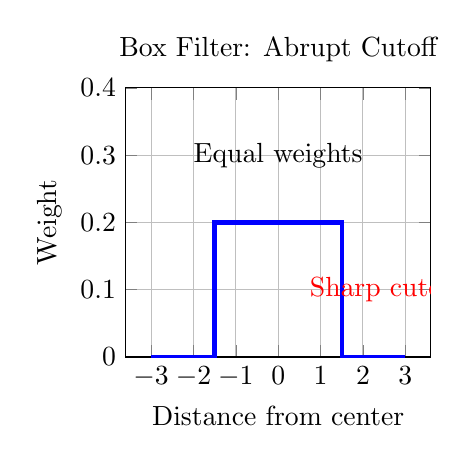
\begin{tikzpicture}
    \begin{axis}[
        width=0.45\textwidth,
        height=5cm,
        xlabel={Distance from center},
        ylabel={Weight},
        title={Box Filter: Abrupt Cutoff},
        ymin=0, ymax=0.4,
        xtick={-3,-2,-1,0,1,2,3},
        grid=major
    ]
    \addplot[color=blue, ultra thick, const plot] coordinates {
        (-3,0) (-1.5,0) (-1.5,0.2) (1.5,0.2) (1.5,0) (3,0)
    };
    \node at (axis cs:0,0.3) {Equal weights};
    \node[red] at (axis cs:2.5,0.1) {Sharp cutoff};
    \end{axis}
\end{tikzpicture}
\hfill
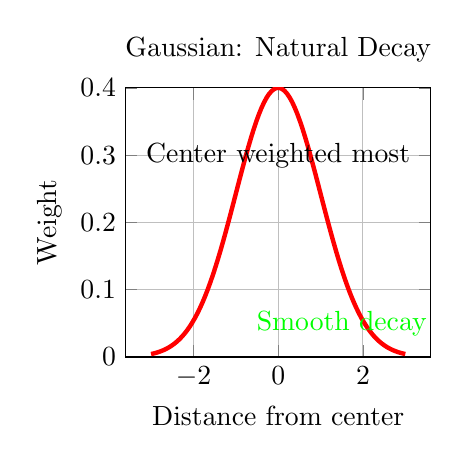
\begin{tikzpicture}
    \begin{axis}[
        width=0.45\textwidth,
        height=5cm,
        xlabel={Distance from center},
        ylabel={Weight},
        title={Gaussian: Natural Decay},
        ymin=0, ymax=0.4,
        domain=-3:3,
        samples=100,
        grid=major
    ]
    \addplot[color=red, ultra thick] {0.4*exp(-x^2/2)};
    \node at (axis cs:0,0.3) {Center weighted most};
    \node[green] at (axis cs:1.5,0.05) {Smooth decay};
    \end{axis}
\end{tikzpicture}
\caption{Gaussian implements a more natural notion of locality}
\end{figure}

\begin{tcolorbox}[colback=yellow!5!white, colframe=orange!50!black, title=Locality Refinement]
The Gaussian kernel implements ``soft'' locality:
\begin{itemize}
    \item Immediate neighbors matter most
    \item Influence decays smoothly with distance
    \item No artificial boundary artifacts
    \item Still translation equivariant!
\end{itemize}
\end{tcolorbox}

\subsection{From Smoothing to Structure - Finding Features}

\paragraph{Derivatives Detect Changes}

To find edges and features, we need to detect \emph{changes} in the signal:

\begin{figure}[h]
\centering
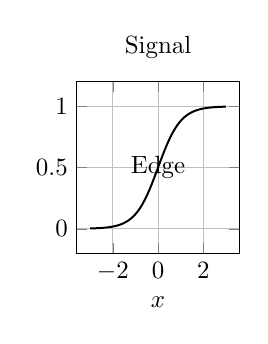
\begin{tikzpicture}[scale=0.9]
    \begin{axis}[
        width=0.32\textwidth,
        height=4cm,
        xlabel={$x$},
        title={Signal},
        grid=major,
        ymin=-0.2, ymax=1.2
    ]
    \addplot[thick, black, domain=-3:3, samples=100] {1/(1+exp(-2*x))};
    \node at (axis cs:0,0.5) {Edge};
    \end{axis}
\end{tikzpicture}
\hfill
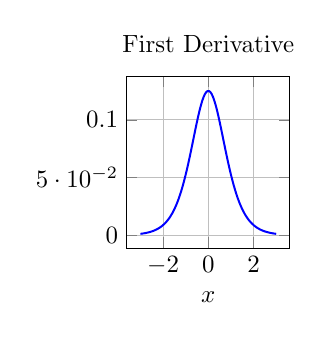
\begin{tikzpicture}[scale=0.9]
    \begin{axis}[
        width=0.32\textwidth,
        height=4cm,
        xlabel={$x$},
        title={First Derivative},
        grid=major
    ]
    \addplot[thick, blue, domain=-3:3, samples=100] {0.5*exp(-2*x)/(1+exp(-2*x))^2};
    \node[blue] at (axis cs:0,0.25) {Peak!};
    \end{axis}
\end{tikzpicture}
\hfill
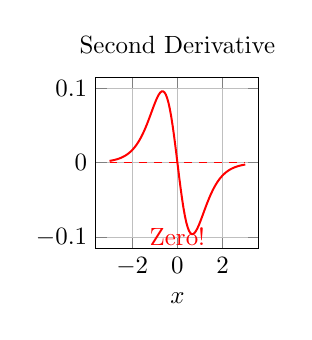
\begin{tikzpicture}[scale=0.9]
    \begin{axis}[
        width=0.32\textwidth,
        height=4cm,
        xlabel={$x$},
        title={Second Derivative},
        grid=major
    ]
    \addplot[thick, red, domain=-3:3, samples=100] {exp(-2*x)*(exp(-2*x)-1)/(1+exp(-2*x))^3};
    \node[red] at (axis cs:0,-0.1) {Zero!};
    \draw[dashed, red] (-3,0) -- (3,0);
    \end{axis}
\end{tikzpicture}
\caption{Derivatives reveal structure: edges appear as peaks or zero crossings}
\end{figure}

\paragraph{The Mexican Hat: A Natural Feature Detector}

The Mexican Hat combines Gaussian smoothing with second derivative detection:

\begin{figure}[h]
\centering
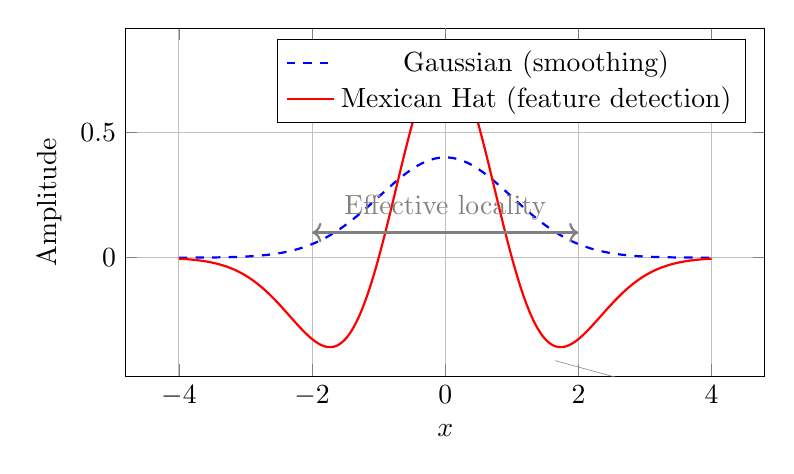
\begin{tikzpicture}
    \begin{axis}[
        width=0.8\textwidth,
        height=6cm,
        xlabel={$x$},
        ylabel={Amplitude},
        domain=-4:4,
        samples=200,
        grid=major,
        legend pos=north east
    ]
    % Components
    \addplot[thick, blue, dashed] {0.4*exp(-x^2/2)};
    \addlegendentry{Gaussian (smoothing)}
    
    \addplot[thick, red] {0.8*(1-x^2)*exp(-x^2/2)};
    \addlegendentry{Mexican Hat (feature detection)}
    
    % Annotations
    \node[red, pin={[red]90:Detects bright blobs}] at (axis cs:0,0.8) {};
    \node[red, pin={[red]-45:Suppresses uniform regions}] at (axis cs:1.5,-0.4) {};
    
    % Show it's still local
    \draw[<->, thick, gray] (axis cs:-2,0.1) -- (axis cs:2,0.1);
    \node[gray] at (axis cs:0,0.2) {Effective locality};
    \end{axis}
\end{tikzpicture}
\caption{The Mexican Hat: local feature detection through derivatives}
\end{figure}



\begin{figure}[h]
\centering
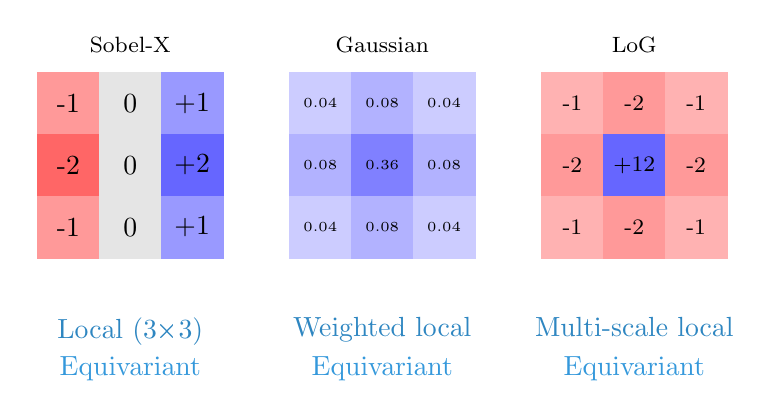
\begin{tikzpicture}[scale=0.8]
    % Sobel X
    \matrix[matrix of nodes, nodes={minimum size=0.8cm, anchor=center}, 
            row sep=-\pgflinewidth, column sep=-\pgflinewidth,
            label={[font=\footnotesize]above:Sobel-X}] (SX) at (0,0) {
        |[fill=red!40]| -1 & |[fill=gray!20]| 0 & |[fill=blue!40]| +1 \\
        |[fill=red!60]| -2 & |[fill=gray!20]| 0 & |[fill=blue!60]| +2 \\
        |[fill=red!40]| -1 & |[fill=gray!20]| 0 & |[fill=blue!40]| +1 \\
    };
    \node[below=0.5cm of SX, locality] {Local (3×3)};
    \node[below=1cm of SX, equivariance] {Equivariant};
    
    % Gaussian
    \matrix[matrix of nodes, nodes={minimum size=0.8cm, anchor=center, font=\tiny}, 
            row sep=-\pgflinewidth, column sep=-\pgflinewidth,
            label={[font=\footnotesize]above:Gaussian}] (GAUSS) at (4,0) {
        |[fill=blue!20]| 0.04 & |[fill=blue!30]| 0.08 & |[fill=blue!20]| 0.04 \\
        |[fill=blue!30]| 0.08 & |[fill=blue!50]| 0.36 & |[fill=blue!30]| 0.08 \\
        |[fill=blue!20]| 0.04 & |[fill=blue!30]| 0.08 & |[fill=blue!20]| 0.04 \\
    };
    \node[below=0.5cm of GAUSS, locality] {Weighted local};
    \node[below=1cm of GAUSS, equivariance] {Equivariant};
    
    % LoG
    \matrix[matrix of nodes, nodes={minimum size=0.8cm, anchor=center, font=\footnotesize}, 
            row sep=-\pgflinewidth, column sep=-\pgflinewidth,
            label={[font=\footnotesize]above:LoG}] (LOG) at (8,0) {
        |[fill=red!30]| -1 & |[fill=red!40]| -2 & |[fill=red!30]| -1 \\
        |[fill=red!40]| -2 & |[fill=blue!60]| +12 & |[fill=red!40]| -2 \\
        |[fill=red!30]| -1 & |[fill=red!40]| -2 & |[fill=red!30]| -1 \\
    };
    \node[below=0.5cm of LOG, locality] {Multi-scale local};
    \node[below=1cm of LOG, equivariance] {Equivariant};
\end{tikzpicture}
\caption{Classical filters: all implement locality and equivariance}
\end{figure}


\subsection{Wavelet Transform via Convolution with the Mexican Hat Kernel}

The \emph{Continuous Wavelet Transform} (CWT) of a signal \(x(t)\) at scale \(a\) and shift \(b\) is given by:
\[
W_x(a,b) = \frac{1}{\sqrt{|a|}} \int_{-\infty}^{\infty} x(t)\,\psi\!\left(\frac{t-b}{a}\right)\,\mathrm{d}t
\]
where \(\psi\) is the mother wavelet (often real‐valued in this case). This is precisely a convolution:
\[
W_x(a,b) = (x * \psi_a)(b)
\]
with \(\psi_a(t) = \frac{1}{\sqrt{|a|}}\psi\left(\frac{t}{a}\right)\).


\paragraph{Mexican Hat (Ricker) Wavelet}

Define the Mexican Hat wavelet \(\psi(t)\) as (up to normalization constant):
\[
\psi(t) = \left(1 - t^2\right)\exp\!\left(-\frac{t^2}{2}\right)
\]
which is the negative normalized second derivative of a Gaussian (also known as the Ricker wavelet or DOG with \(m=2\)).

Scaled and shifted:
\[
\psi_{a,b}(t) = \frac{1}{\sqrt{|a|}}\,\psi\!\left(\frac{t - b}{a}\right)
\]
so the wavelet transform becomes:
\[
W_x(a,b) \;=\; \int x(t)\,\psi_{a,b}(t)\,\mathrm{d}t = (x * \psi_{a})(b).
\]

\paragraph{Intuition of Convolution with Mexican Hat}

- Convolution with \(\psi_{a}\) acts as a \emph{localized band-pass filter} extracting structures in \(x(t)\) whose width matches scale \(a\).
- The Mexican Hat wavelet, being second derivative of a Gaussian, responds strongly to \emph{peaks or dips} (inflection‐points) in the signal at that scale.
- As you vary \(a\), you sweep across time–frequency features: small \(a\) captures high‐frequency, narrow-scale changes; large \(a\) broad, low‐frequency structures.:contentReference[oaicite:4]{index=4}


\[
W_x(a,b)
= \int_{-\infty}^\infty x(t)\,\psi_{a,b}(t)\,\mathrm{d}t
= (x * \psi_a)(b),
\quad
\psi(t) = (1 - t^2) e^{-t^2/2}
\]







\section{The Linear Algebra of Convolution: Circulant Matrices and the FFT}\label{app:circulant}

This appendix provides the mathematical foundations for why convolution is so fundamental and computationally efficient and is based on Chapter ? of Gil Strang book \cite{}.

\begin{tcolorbox}[colback=yellow!5!white, colframe=orange!50!black, title=The Big Picture]
Understanding the matrix structure of convolution reveals:
\begin{itemize}
    \item Why CNNs have far fewer parameters than fully-connected networks
    \item How the FFT makes large convolutions practical
    \item The deep connection between spatial operations and frequency analysis
    \item Why convolution is the ``natural'' operation for spatial data
\end{itemize}
\end{tcolorbox}

\subsection{From Shift Operations to Circulant Matrices}

\paragraph{The Shift Matrix}

Consider the cyclic shift matrix:
\[
P = \begin{bmatrix}
0 & 1 & 0 & \cdots & 0 \\
0 & 0 & 1 & \cdots & 0 \\
\vdots & \vdots & \vdots & \ddots & \vdots \\
0 & 0 & 0 & \cdots & 1 \\
1 & 0 & 0 & \cdots & 0
\end{bmatrix}
\]

This matrix shifts vectors cyclically:
\[
P \begin{bmatrix} x_0 \\ x_1 \\ x_2 \\ x_3 \end{bmatrix} = \begin{bmatrix} x_1 \\ x_2 \\ x_3 \\ x_0 \end{bmatrix}
\]

Key properties:
\begin{itemize}
    \item $P^k$ shifts by $k$ positions
    \item $P^n = I$ (after $n$ shifts, we return to start)
    \item $P$ generates all cyclic translations
\end{itemize}

\paragraph{Circulant Matrices as Polynomials in $P$}

\begin{theorem}[Fundamental Characterization]
A matrix $C$ is circulant if and only if it can be written as:
\[
C = c_0 I + c_1 P + c_2 P^2 + \cdots + c_{n-1} P^{n-1}
\]
\end{theorem}

This gives the familiar structure where each row is a cyclic shift of the previous:
\[
C = \begin{bmatrix}
c_0 & c_1 & c_2 & \cdots & c_{n-1} \\
c_{n-1} & c_0 & c_1 & \cdots & c_{n-2} \\
c_{n-2} & c_{n-1} & c_0 & \cdots & c_{n-3} \\
\vdots & \vdots & \vdots & \ddots & \vdots \\
c_1 & c_2 & c_3 & \cdots & c_0
\end{bmatrix}
\]

\begin{figure}[h]
\centering
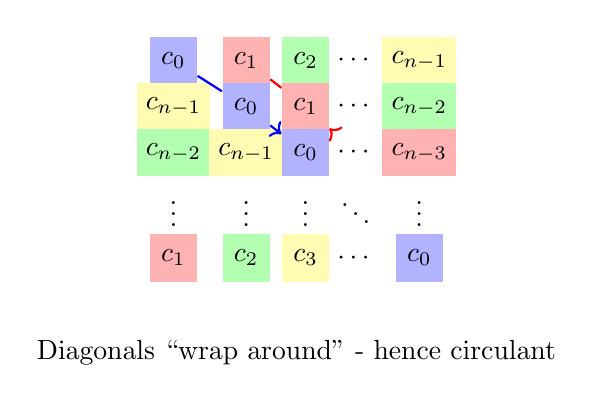
\begin{tikzpicture}[scale=0.8]
    % Matrix with diagonal pattern
    \matrix[matrix of nodes, nodes={minimum size=0.6cm, anchor=center}, 
            row sep=-\pgflinewidth, column sep=-\pgflinewidth] (M) {
        |[fill=blue!30]| $c_0$ & |[fill=red!30]| $c_1$ & |[fill=green!30]| $c_2$ & $\cdots$ & |[fill=yellow!30]| $c_{n-1}$ \\
        |[fill=yellow!30]| $c_{n-1}$ & |[fill=blue!30]| $c_0$ & |[fill=red!30]| $c_1$ & $\cdots$ & |[fill=green!30]| $c_{n-2}$ \\
        |[fill=green!30]| $c_{n-2}$ & |[fill=yellow!30]| $c_{n-1}$ & |[fill=blue!30]| $c_0$ & $\cdots$ & |[fill=red!30]| $c_{n-3}$ \\
        $\vdots$ & $\vdots$ & $\vdots$ & $\ddots$ & $\vdots$ \\
        |[fill=red!30]| $c_1$ & |[fill=green!30]| $c_2$ & |[fill=yellow!30]| $c_3$ & $\cdots$ & |[fill=blue!30]| $c_0$ \\
    };
    
    % Diagonal arrows
    \draw[thick, blue, ->] (M-1-1) -- (M-2-2) -- (M-3-3);
    \draw[thick, red, ->] (M-1-2) -- (M-2-3) -- (M-3-4);
    
    \node[below=0.5cm of M] {Diagonals ``wrap around'' - hence circulant};
\end{tikzpicture}
\end{figure}

\subsection{The Fourier Connection}

\paragraph{Eigenvectors of Circulant Matrices}

\begin{theorem}[Shared Eigenvectors]
All circulant matrices share the same eigenvectors - the columns of the Fourier matrix:
\[
\mathbf{q}_k = \frac{1}{\sqrt{n}} \begin{bmatrix} 1 \\ \omega^k \\ \omega^{2k} \\ \vdots \\ \omega^{(n-1)k} \end{bmatrix}, \quad \text{where } \omega = e^{2\pi i/n}
\]
\end{theorem}

\begin{proof}[Proof Sketch]
For the shift matrix $P$:
\[
P\mathbf{q}_k = P \begin{bmatrix} 1 \\ \omega^k \\ \omega^{2k} \\ \vdots \\ \omega^{(n-1)k} \end{bmatrix} = \begin{bmatrix} \omega^k \\ \omega^{2k} \\ \vdots \\ \omega^{(n-1)k} \\ 1 \end{bmatrix} = \omega^k \begin{bmatrix} 1 \\ \omega^k \\ \omega^{2k} \\ \vdots \\ \omega^{(n-1)k} \end{bmatrix} = \omega^k \mathbf{q}_k
\]
Since $\omega^{nk} = 1$. Thus $\mathbf{q}_k$ is an eigenvector with eigenvalue $\omega^k$.
\end{proof}

\paragraph{Eigenvalues and the DFT}

For a circulant matrix $C = \sum_{j=0}^{n-1} c_j P^j$, the eigenvalue corresponding to $\mathbf{q}_k$ is:
\[
\lambda_k = c_0 + c_1 \omega^k + c_2 \omega^{2k} + \cdots + c_{n-1} \omega^{(n-1)k}
\]

This is exactly the $k$-th component of the Discrete Fourier Transform of $(c_0, c_1, \ldots, c_{n-1})$!

\subsection{The Convolution Theorem}

\begin{theorem}[Convolution Rule]
Let $\mathbf{x}$ and $\mathbf{h}$ be vectors and $\mathbf{y} = \mathbf{x} \circledast \mathbf{h}$ their cyclic convolution. Then:
\[
\mathcal{F}(\mathbf{y}) = \mathcal{F}(\mathbf{x}) \odot \mathcal{F}(\mathbf{h})
\]
where $\mathcal{F}$ is the DFT and $\odot$ is element-wise multiplication.
\end{theorem}

This leads to the FFT algorithm for convolution:
\begin{enumerate}
    \item Compute $\mathcal{F}(\mathbf{x})$ and $\mathcal{F}(\mathbf{h})$ using FFT: $O(n \log n)$
    \item Element-wise multiply: $O(n)$
    \item Inverse FFT: $O(n \log n)$
\end{enumerate}
Total: $O(n \log n)$ instead of $O(n^2)$ for direct convolution!

\subsection{From Cyclic to Linear Convolution}

\paragraph{Boundary Conditions Matter}

In practice, we use different boundary conditions:
\begin{itemize}
    \item \textbf{Circular/Periodic}: Wraparound $\rightarrow$ Circulant matrix
    \item \textbf{Zero padding}: Pad with zeros $\rightarrow$ Toeplitz matrix
    \item \textbf{Reflection}: Mirror at boundaries $\rightarrow$ Modified Toeplitz
\end{itemize}

\begin{figure}[h]
\centering
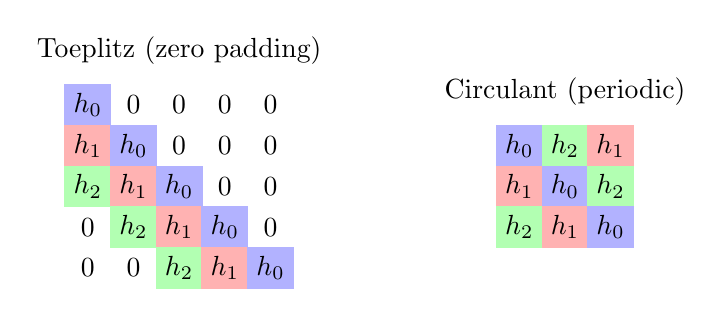
\begin{tikzpicture}[scale=0.7]
    % Toeplitz structure
    \matrix[matrix of nodes, nodes={minimum size=0.5cm, anchor=center}, 
            row sep=-\pgflinewidth, column sep=-\pgflinewidth,
            label=above:Toeplitz (zero padding)] (T) at (0,0) {
        |[fill=blue!30]| $h_0$ & 0 & 0 & 0 & 0 \\
        |[fill=red!30]| $h_1$ & |[fill=blue!30]| $h_0$ & 0 & 0 & 0 \\
        |[fill=green!30]| $h_2$ & |[fill=red!30]| $h_1$ & |[fill=blue!30]| $h_0$ & 0 & 0 \\
        0 & |[fill=green!30]| $h_2$ & |[fill=red!30]| $h_1$ & |[fill=blue!30]| $h_0$ & 0 \\
        0 & 0 & |[fill=green!30]| $h_2$ & |[fill=red!30]| $h_1$ & |[fill=blue!30]| $h_0$ \\
    };
    
    % Circulant structure
    \matrix[matrix of nodes, nodes={minimum size=0.5cm, anchor=center}, 
            row sep=-\pgflinewidth, column sep=-\pgflinewidth,
            label=above:Circulant (periodic)] (C) at (7,0) {
        |[fill=blue!30]| $h_0$ & |[fill=green!30]| $h_2$ & |[fill=red!30]| $h_1$ \\
        |[fill=red!30]| $h_1$ & |[fill=blue!30]| $h_0$ & |[fill=green!30]| $h_2$ \\
        |[fill=green!30]| $h_2$ & |[fill=red!30]| $h_1$ & |[fill=blue!30]| $h_0$ \\
    };
\end{tikzpicture}
\caption{Toeplitz vs Circulant structure depends on boundary conditions}
\end{figure}

\subsection{2D Extension and CNNs}

\paragraph{Block Structure}

For 2D convolution with circular boundaries:
\begin{itemize}
    \item The matrix is \textbf{Block Circulant with Circulant Blocks} (BCCB)
    \item Diagonalized by 2D DFT: $F \otimes F$ (Kronecker product)
    \item 2D FFT convolution: $O(n^2 \log n)$ vs $O(n^4)$ direct
\end{itemize}


Modern CNNs typically use:
\begin{itemize}
    \item \textbf{Valid} or \textbf{same} convolution (not circular)
    \item Small kernels (3×3, 5×5) where direct computation is often faster
    \item Multiple channels: tensor operations, not just matrix multiplication
\end{itemize}

Parameter count for a conv layer:
\[
\text{\# params} = k_h \times k_w \times C_{in} \times C_{out} + C_{out}
\]
This is independent of image size - the power of weight sharing!

\paragraph{Why Convolution Works for Spatial Data}

\begin{theorem}[Fundamental Result]
Any linear operator that commutes with translations must be a convolution.
\end{theorem}

This theorem explains why convolution is natural for images:
\begin{enumerate}
    \item Images have translation symmetry (objects can appear anywhere)
    \item We want features that respect this symmetry (equivariance)
    \item Mathematics forces us to use convolution!
\end{enumerate}

\subsection{Practical Example: Speed Comparison}

\begin{center}
\begin{tabular}{|c|c|c|c|}
\hline
Signal Length & Direct Conv & FFT Conv & Speedup \\
\hline
128 & 16,384 ops & 896 ops & 18× \\
512 & 262,144 ops & 4,608 ops & 57× \\
2048 & 4,194,304 ops & 22,528 ops & 186× \\
\hline
\end{tabular}
\end{center}

\paragraph{Summary:}

The circulant matrix perspective reveals:
\begin{itemize}
    \item \textbf{Weight sharing} = Structured matrix with repeated diagonals
    \item \textbf{Translation equivariance} = Commuting with shift operations
    \item \textbf{Fourier diagonalization} = Why FFT accelerates convolution
    \item \textbf{Parameter efficiency} = $O(n)$ parameters vs $O(n^2)$ for fully connected
\end{itemize}

This mathematical framework explains why CNNs are both theoretically principled and computationally efficient for spatial data processing.


\section{ 1x1 convolution}

A 1x1 convolution is a powerful and efficient tool in neural networks. While it doesn't look at neighboring data points like larger convolutions do, it performs a crucial role by operating across the channels (also called filters) of the data.

In this generator model, the 1x1 convolutions have two primary functions:

Changing the Number of Channels (Dimensionality Reduction): This is its main job in this diagram. The network progressively reduces the number of channels from 512 down to 256, then to 128, and finally to 18.  This is a computationally cheap way to decrease the complexity and number of parameters in the network as it gets closer to the final output.


Adding Non-Linearity: Each 1x1 convolutional layer is followed by a Leaky ReLU activation layer.  This combination allows the network to learn complex, non-linear relationships between the channels. Think of it as a small, fully connected network that decides how to mix and recombine the feature information at each step without altering the time-series dimension.


In essence, the 1x1 convolutions in this model act as an efficient feature transformation step, helping the generator refine the abstract information from the latent space and conditional inputs (insulin and carbs) until it has the right shape and complexity to be the final 18-sample blood glucose vector.
\end{document}
